\documentclass[a4paper]{memoir}
% pre'ambulo

\usepackage[latin1]{inputenc}
\usepackage[spanish,activeacute]{babel}
%\usepackage[group-separator={,}]{siunitx}
\usepackage{amsmath}
\usepackage{parskip}
\usepackage{setspace}
\usepackage{url}
\usepackage{graphicx}
\usepackage{booktabs}

\newtheorem{ejem}{Ejemplo}[chapter]
\newtheorem{defi}{Definici�n}[chapter]

\renewcommand{\baselinestretch}{1.5}

\title{Valoraci�n de empresas utilizando computaci�n con palabras}
\author{Manuel L�pez P�rez}

\begin{document}

\spanishdecimal{,}
\def\tablename{Tabla}
\setlength{\parskip}{1.5ex plus 0.5ex minus 0.2ex}

% cuerpo del documento

\maketitle
\newpage
Aqui va la primera p�gina formato UMA
\newpage

\tableofcontents

\part {Introducci�n}
\chapter{Introduccion}
\section{Introducci�n a la valoraci�n de empresas}

La b�squeda del valor de una empresa es un problema com�n que se ha convertido en un pilar b�sico en finanzas. De hecho, el objetivo financiero de cualquier empresa no es otro que maximizar dicho valor. Esta circunstancia ha convertido la valoraci�n de empresas en un desaf�o para cualquier analista o agente. La metodolog�a que facilita la obtenci�n de dicho valor surge de la evoluci�n de la teor�a financiera, siendo su idea fundamental que el valor de los activos es la actualizaci�n de los flujos financieros que es capaz de generar en el futuro.

El valor busca su apoyo en un fundamento l�gico o matem�tico lo m�s riguroso posible. Busca la objetividad, la neutralidad y la independencia frente a las partes, las fuertes relaciones en el mercado, e incluso la propia situaci�n del mercado. Sin embargo, la necesidad de predecir escenarios futuros en los cuales se va a desarrollar la actividad de la misma, am�n de otras circunstancias, genera la imposibilidad de determinar un �nico valor, lo que nos limita a establecer un rango u horquilla de valores posibles, dentro de los cuales se encontrar� el valor m�s probable de la empresa. El valor definitivo vendr� por consenso y/o negociaci�n entre las partes interesadas. En consecuencia, ser� la amplitud de la horquilla de valores posibles la que finalmente caracterice el informe de valoraci�n previo a la decisi�n.

La computaci�n con palabras es un sistema de computaci�n que ofrece una importante capacidad que los sistemas de computaci�n tradicionales no tienen: la capacidad de realizar c�lculos con informaci�n descrita en lenguaje natural. Usando como base la l�gica difusa y el concepto de \emph{etiqueta ling��stica}, veremos como a�adir informaci�n expresada en lenguaje natural al proceso de valoraci�n de empresas. As�, esta valoraci�n se ver� ajustada al tener en cuenta no solo los valores p�ramente cuantitativos, si no adem�s la informaci�n cualitativa provista por un conjunto de expertos respecto a dichos valores num�ricos.

Usando esta herramienta queremos dar un salto de calidad en la mejora de la informaci�n disponible para el inversor, dado que si con la metodolog�a propuesta logramos cerrar la horquilla de valores posibles, acercaremos las posturas de las partes interesadas. Si lo conseguimos, habremos aumentado la posibilidad de acuerdo en cerrar la operaci�n en un precio de equilibrio consensuado o m�nimamente negociado. De esta forma habremos colaborado al aumento de la liquidez y eficiencia del mercado.

\section{Objetivos del proyecto}

El objetivo principal es la implementaci�n algor�tmica de dos m�todos de valoraci�n de empresas usando computaci�n con palabras. Por un lado, el denominado \emph{M�todo de flujos descontados (Discounted Cash-flow) con operadores OWA}\cite{Cashflow1} y por otro el \emph{M�todo de An�lisis Mixto o M�todo operativo con operadores OWA}\cite{Expertones1}. Estos m�todos hacen uso de computaci�n con palabras a trav�s del concepto de \emph{Mayor�a Ling��stica} y el operador $LAMA$, que es uno de los denominados \emph{operadores de agregaci�n OWA (Ordered Weight Averaging)}.

Con la implementaci�n obtenida procederemos a la realizaci�n de una bater�a de pruebas automatizada, de forma que podamos obtener resultados comparativos de ambos m�todos, dilucidando cual nos da horquillas de valoraci�n m�s ajustadas en cada caso.

As� mismo, se implementar� una interfaz de usuario para la ejecuci�n de casos de ejemplo con ambos m�todos, facilitando la entrada de datos de forma sencilla e intuitiva, y que muestre los resultados obtenidos de forma comparativa, clara y concisa a cualquier usuario. 

\section{Estructura de la memoria}

Para la presentaci�n del proyecto estructuraremos la presente memoria en X cap�tulos y dos ap�ndices, comenzando por este cap�tulo de introducci�n.

En el cap�tulo dos trataremos de forma m�s extensa la problem�tica de la valoraci�n de empresas, incidiendo en la importancia de la inclusi�n de informaci�n cualitativa en el proceso de valoraci�n. Por �ltimo introduciremos los conceptos de l�gica difusa y computaci�n con palabras aplicados a la valoraci�n de empresas.

En el tercer cap�tulo introduciremos los conceptos matem�ticos necesarios para el desarrollo de los m�todos de valoraci�n que utilizan computaci�n con palabras. Presentaremos el modelo de 2-tuplas para la representaci�n de la informaci�n ling��stica y el concepto de mayor�a. Tambi�n introduciremos el m�todo de los Expertones, que es otro modo, distinto al concepto de \emph{mayor�a ling��stica}, para introducir informaci�n cualitativa en la valoraci�n de empresas. Por �ltimo presentaremos los m�todos "`sin mayor�a"' de valoraci�n de empresas, que luego modificaremos utilizando computaci�n con palabras. Estos son el m�todo de Flujos descontados (Cash-flow) y el m�todo de An�lisis Mixto u Operativo.

En el cuarto cap�tulo presentaremos, de forma conceptual, los modelos de valoraci�n de empresas. Primero en su forma original, y despu�s modificados convenientemente para incluir la informaci�n cualitativa utilizando el concepto de Mayor�a, mostrando un ejemplo de utilizaci�n para cada modelo. 

En el quinto cap�tulo trataremos la implementaci�n de dichos modelos, as� como de la bater�a de pruebas a ejecutar sobre ellos, desde el punto de vista de la ingenier�a del software, introduciendo el an�lisis funcional y t�cnico utilizando diagramas UML.

En el sexto cap�tulo trataremos sobre la bater�a de pruebas realizada y sus resultados, para obtener una comparativa de ambos m�todos. Analizaremos los resultados obtenidos para discernir en qu� casos es mejor utilizar cada m�todo y discutiremos las ventajas e inconvenientes de cada uno.

Por �ltimo se incluir� un cap�tulo de conclusiones, en el que adem�s sugeriremos futuros trabajos a realizar, ya sean mejoras sobre la implementaci�n de los m�todos de valoraci�n como posibles mejoras o ampliaciones de la funcionalidad de la interfaz de usuario.

Adem�s se incluir�n como ap�ndices los manuales de instalaci�n y uso del software, as� como la bibliograf�a utilizada para la realizaci�n del proyecto.

\part {Conceptos previos}
\chapter{Introducci�n a la valoraci�n de empresas}

\section{Introducci�n}

En este cap�tulo estudiaremos m�s a fondo la problem�tica de la valoraci�n de empresas. Estudiaremos las causas que impiden que el valor de una empresa sea un valor absoluto y veremos adem�s la importancia de la informaci�n cuantitativa en el escenario de incertidumbre en el que se llevan a cabo los procesos de valoraci�n. 

Por �ltimo introduciremos brevemente los dos m�todos de valoraci�n que utilizaremos en este proyecto.

\section{La problem�tica de la valoraci�n de empresas}
Podemos decir que una empresa vale, como cualquier otro elemento susceptible de ser comprado o vendido, el precio que alguien est� dispuesto a pagar por ella. Esta afirmaci�n, que es totalmente obvia, recoge, sin embargo, una verdad absoluta sobre el valor de una empresa: que �ste es totalmente subjetivo. Es decir, al contrario que pasa con otros elementos en la vida, no existe un valor objetivo, definitivo y absoluto, de una empresa, una cifra que nadie pudiera discutir y de la que se pudiera afirmar sin lugar a dudas: "`esta empresa vale esta cantidad."'

Una empresa no es algo que pueda medirse ("`100 metros"') o pesarse ("`10 toneladas"') con absoluta certeza del resultado. Una empresa puede tener activos perfectamente medibles sin que su menci�n d� lugar a dudas, como por ejemplo un almac�n de 1.000 metros cuadrados. Pero aun as�, la conversi�n en dinero de esos activos ya empezar� a ser relativa. 

Una empresa, por tanto, puede tener muchos valores distintos, dependiendo de quien la valora, y de la perspectiva con que lo hace. Es decir, no es lo mismo valorar para comprar que valorar para vender, ni es lo mismo valorar para liquidar que valorar para mantener la empresa viva a largo plazo, ni para mantenerla independiente que para integrarla en un grupo empresarial mayor, por ejemplo. En conclusi�n: el valor de una empresa es relativo, depende de quien la valora y de para qu� la valora. Incluso tambi�n depende del momento en que se la valora. \emph{Existen tantos valores de una empresa como personas distintas la est�n valorando o momentos distintos en que se la valore.}

El valor de una empresa en funcionamiento depende principalmente de las expectativas que el que la valora tenga de los beneficios futuros que la empresa va a dar. Y cuando hablamos de expectativas, como concepto esencialmente subjetivo que es, podr�amos decir que no hay dos expectativas iguales, porque cada persona tiene las suyas, y m�s cuando se trata de imaginar c�mo va a evolucionar en el futuro un panorama de variables tan complejo como el que rodea a una empresa: el mercado en el que vende y compra, sus precios, sus costes, sus competidores, su personal, los avances tecnol�gicos que le afectan, la legislaci�n, los gustos de los clientes, etc. Por tanto, es importante entender que, a la hora de ponerse de acuerdo, cuando discutan de precio el comprador y el vendedor de una empresa, en realidad van a estar discutiendo b�sicamente de expectativas. Sean conscientes de ello o no, aunque parezca que est�n discutiendo de cifras de presente, o de pasado, en realidad est�n discutiendo de cifras y expectativas de futuro. 

Toda empresa no vale hoy por lo que lleg� a valer en el pasado, sino por lo que valdr� en un futuro. Es cierto que detr�s del c�lculo del valor de una empresa puede haber un sinf�n de f�rmulas de matem�ticas financieras, que determinen el valor actual de los flujos de fondos futuros a una determinada tasa de descuento, teniendo en cuenta el coste del dinero sin riesgo m�s una tasa de riesgo, y que ponerse de acuerdo sobre esa tasa de descuento no es tarea f�cil; pero lo que realmente cuenta es ponerse primero de acuerdo sobre la magnitud de los flujos futuros de beneficios que comprador y vendedor creen que se pueden obtener de esa empresa. La transacci�n no se llevar� a cabo hasta que ambos vean las mismas cifras, o, mejor dicho, cuando el comprador vea o crea ver, aunque no lo diga, flujos de beneficios mayores de los que est� considerando el vendedor. Es entonces cuando se produce la compraventa. De hecho, aunque parezca sorprendente, en el fondo, si fuera cierto que ambos vieran exactamente los mismos beneficios futuros, lo m�s probable es que la venta no se produjese, porque el vendedor le pedir�a al comprador exactamente lo que �ste estuviera pensando que val�a la empresa, y entonces el comprador no ganar�a nada compr�ndola, por lo que, en buena l�gica, no la comprar�a. Como en cualquier proceso de compra de un bien o servicio, es cuando el comprador tiene la sensaci�n de estar comprando algo a un precio por debajo del valor que lo que est� comprando tiene para �l, cuando se produce la compraventa. Y viceversa para el caso del vendedor; �ste vende cuando piensa que lo que est� vendiendo vale menos que lo que le van a pagar.\cite{LopezMartinez1}

Por tanto, debido a todos estos factores subjetivos y de incertidumbre, es imposible determinar un �nico valor para una empresa. Cuando valoramos una empresa intentamos determinar un intervalo de valores razonables en el cual se encontrar� el valor definitivo de la empresa. Cuanto m�s peque�a sea la amplitud de dicho intervalo, m�s facil ser� para las partes implicadas en la negociaci�n alcanzar un acuerdo final, aumentando as� la eficiencia del mercado. 


\section{La importancia de la informaci�n cualitativa}

Hemos visto que hay un alto componente subjetivo en todo el proceso de valoracion de empresas. Adem�s, el hecho de que la valoraci�n dependa en gran medida de la estimaci�n del valor futuro supone que la decisi�n se toma siempre en un escenario de incertidumbre, dado que, por completos que sean los datos de los que dispongamos, no existe una manera cient�fica de predecir el futuro. 

Esto nos lleva a que para cualquier proceso de valoraci�n ser� necesario establecer una estimaci�n de los distintos par�metros que influir�n determinantemente en la horquilla de valores. Esta estimaci�n, por otra parte, nunca ser� unica, ni se tratar� de valores exactos, ya que depender� de la situaci�n de la empresa, el momento en que se realice la valoraci�n, y el m�todo usado para �sta. 

En muchos casos, estas estimaciones son expresadas por distintos expertos en funci�n a su experiencia previa y su percepci�n de la realidad. y que en muchos casos se definen con t�rminos linguisticos y con diferentes dominios de expresi�n. Esto es, un experto puede dar su opini�n en t�rminos simplemente de "`mucho"', "`poco"' y "`nada"' mientras que otro experto puede dar su opini�n en un dominio m�s �mplio que abarque t�rminos como "`m�ximo"', "`mucho"', "`termino medio"', "`poco"', "`muy poco"' y "`nada"'. As� que, mientras para el primer �xperto el t�rmino "`mucho"' representar�a el m�ximo posible, para el segundo experto el mismo t�rmino expresar�a un grado m�s bajo, al poder usar la expresi�n "`m�ximo"' para representar el mayor grado de su opini�n.

En estas condiciones es necesario tener herramientas que permitan operar con la incertidumbre y la inexactitud de las opiniones expresadas. Adem�s, estas herramientas deben ser capaces de a�adir dichas opiniones de forma representativa. Es decir, si la mayor�a de estimaciones apunta hacia un valor alto, al a�adir la informaci�n al proceso de valoraci�n deber� verse reflejada obteniendo una valoraci�n m�s alta. Si en cambio las estimaciones est�n repartidas de forma dispersa, algunas apuntando un valor al alza y otras apuntando un valor a la baja, al a�adir la informaci�n al proceso de valoraci�n �ste no deber�a verse apenas influenciado, puesto que debido a la diversidad de opiniones, ninguna tendr� un peso demasiado elevado que pueda influir en la valoraci�n final. 

Por tanto, al movernos en un escenario de incertidumbre, tenemos gran cantidad de informaci�n \emph{cualitativa}, dependiente de opiniones y expresada en t�rminos ling��sticos, en contraposici�n a la informaci�n \emph{cuantitativa}, que es absoluta y podemos expresar con n�meros. 

Para la introducci�n de estos valores cuantitativos o num�ricos en el proceso de valoraci�n de una empresa existen varios m�todos bien definidos. En este trabajo utilizaremos dos de ellos: el \emph{m�todo de flujos de caja descontados}, m�s conocido por su nombre en ingl�s \emph{Discounted Cash-Flow}, y el \emph{m�todo de an�lisis mixto u an�lisis operativo}, que explicaremos a continuaci�n.

Para a�adir la informaci�n cuantitativa, utilizaremos la computaci�n con palabras y el concepto de \emph{mayor�a ling��stica}, que se basan en la \emph{l�gica difusa}. A continuaci�n haremos una breve introducci�n a estos conceptos, que estudiaremos con m�s profundidad en el siguiente cap�tulo.

\section{M�todos de valoraci�n de empresas}

Aunque el estudio a fondo de los m�todos de valoraci�n de empresas queda fuera de los objetivos de este proyecto, introduciremos brevemente los dos m�todos a utilizar y sobre los que en los siguiente cap�tulos a�adiremos la informaci�n cualitativa usando computaci�n con palabras. 

Se han ofrecido diversas alternativas parar realizar el proceso de valoraci�n entre los que destacan los siguientes:

\textit{Criterio del precio hist�rico}: Se basa en considerar como valor de cada elemento del activo el precio por el que se adquiri� en el momento de su incorporaci�n a la empresa, presentando por tanto claros inconvenientes al no considerar el efecto de la inflaci�n, del progreso t�cnico, etc.

\textit{Criterio del valor de reposici�n}: Este criterio toma como referencia en la estimaci�n de los precios de cada una de las masas patrimoniales del activo su situaci�n actual en el mercado y su eficiencia econ�mica.

\textit{Criterio del beneficio capitalizado}: Parte de la premisa de la obtenci�n de beneficios como objetivo prioritario de la empresa, siendo estos �ltimos la base para el c�lculo del valor de la empresa. De ah�, que la valoraci�n se realice descontando, mediante el tipo de inter�s, los beneficios estimados para periodos futuros, siendo preciso establecer tres variables: tipo de inter�s, beneficios para cada periodo y tiempo que se considera para el an�lisis.

El proceso de valoraci�n realizado en funci�n de este �ltimo criterio debe suponer un valor superior al realizado sobre la base del resto de criterios, denomin�ndose la diferencia \emph{fondo de comercio} o \emph{goodwill}, cuyo c�lculo se afronta desde dos perspectivas principales: el m�todo directo que consiste en estimar unos beneficios posibles y unos beneficios normales actualizando la diferencia, y el m�todo indirecto que consiste en actualizar la estimaci�n de beneficios y restarle el valor sustancial.

\subsection{M�todos de an�lisis mixto}
El criterio del beneficio capitalizado matizado con el del valor sustancial da lugar a lo que se denominan m�todos mixtos, entre los que destacan el m�todo alem�n, el m�todo de Schmalenbach y el m�todo anglosaj�n. El m�todo alem�n trata de evitar el inconveniente de la incertidumbre de los datos futuros. Para ello, y debido a la inexistencia de t�cnicas apropiadas para realizar su tratamiento, se ha optado por reducir el valor capitalizado a la mitad del goodwill tomando como justificaci�n el principio de prudencia valorativa. De esta forma, se tiene que:
\begin{equation}
	V_{e} = V_{s} + \frac{1}{2}GW = V_{c} - \frac{1}{2}GW = V_{c} - \frac{1}{2}(V_{c}-V_{s}) = \frac{V_{c}-V_{s}}{2}
	\label{eq:goodwill}
\end{equation}

Donde $V_{e}$ es el valor de la empresa, $V_{s}$ es el valor sustancial, $V_{c}$ es el valor capitalizado, y $GW$ el \textit{goodwill} $\left(V_{c}-V_{s}\right)$.

En la expresi�n anterior se puede observar que este m�todo determina el valor de la empresa como la media entre el valor capitalizado y el valor sustancial, considerando en consecuencia la misma importancia para ambos tipos de valores.

Por su parte, el m�todo anglosaj�n realiza el c�lculo a�adiendo al valor sustancial el importe total del goodwill. En consecuencia, ambos m�todos adolecen de similares limitaciones, ya que var�a �nicamente el procedimiento de c�lculo, mientras que en el m�todo alem�n el goodwill se obtiene indirectamente como diferencia entre el valor capitalizado y el valor sustancial; por su parte, el m�todo anglosaj�n lo obtiene directamente actualizando la diferencia entre los beneficios esperados y los rendimientos normales del valor sustancial, con lo cual, siendo \emph{i} el tipo de inter�s normal, el valor de la empresa vendr� dado por:

\begin{equation}
	V_{e} = V_{s} + \left(B+iV_{s}\right) \frac{\left(1+i\right)^n - 1}{\left(1+i\right)\cdot i}
	\label{eq:goodwill2}
\end{equation}

La expresi�n anterior refleja el hecho de que los rendimientos normales en lugar de ser calculados sobre el valor sustancial tienen en cuenta el valor de la empresa, denotando lo que te�ricamente pagar�n los eventuales compradores.

En caso de que la estimaci�n de beneficios y tipos de inter�s para los periodos futuros presente distintos valores en cada periodo, el valor de la empresa vendr� determinado por la expresi�n que se recoge a continuaci�n:

\begin{equation}
	\begin{split}
	V_{e} &= V_{s} + \left(B_{1}-i_{1}V_{}s\right)\left(1+i_{1}\right)^{-1} + \cdots \\
	& \cdots+ \left(B_{n}-i_{n}V_{s}\right)\left(1+i_{1}\right)^{-1}\left(1+i_{2}\right)^{-1}\cdots\left(1+i_{n}\right)^{-1}	
	\end{split}
	\label{eq:analisisMixto}	
\end{equation}

Sin embargo, el c�lculo as� efectuado presenta una serie de inconvenientes que es preciso considerar y tratar de evitar para poder establecer una valoraci�n, lo m�s cercana a la realidad posible.

Entre estos inconvenientes est�n la forma en que se expresan las estimaciones y la forma en que se agrega la informaci�n. Tanto las valoraciones de los tipos de inter�s como de los beneficios futuros esperados debe ser realizada por expertos, en cuyo caso se debe establecer un mecanismo que facilite la obtenci�n y posterior agregaci�n de dicha informaci�n. Para la expresi�n de las estimaciones, al no poderse obtener mediante un valor cuantitativo, es m�s factible obtenerla expresada de forma cualitativa para lo que se debe usar un enfoque ling��stico. Adem�s, como se ha indicado anteriormente, es muy importante que el valor agregado sea cercano a la mayor�a de las estimaciones obtenidas por los expertos. Por ello es interesante considerar nuevos operadores que permitan introducir el concepto de mayor�a difusa en la agregaci�n.

\subsection{M�todo de los flujos descontados}

En los �ltimos a�os, con la globalizaci�n de los mercados, el paralelo desarrollo tecnol�gico de los mismos y la aparici�n de nuevos instrumentos financieros, se han desarrollado tambi�n nuevas t�cnicas de valoraci�n y mejorado las existentes. Ello ha llevado consigo un aumento del espectro de m�todos de valoraci�n, de su posible marco de actuaci�n y de la necesidad de discriminar qu� m�todos son aplicables en unas determinadas circunstancias u otras y la veracidad y credibilidad de sus resultados.

En el presente trabajo utilizaremos el m�todo qque en la actualidad tiene mayor aceptaci�n en la comunidad cient�fica y profesional, que no es otro que el modelo de los flujos descontados o \textit{discounted cashflow} por su nombre en ingl��s. La conocida expresi�n general que lo caracteriza es la siguiente:

\begin{equation}
	V_{E} = \sum\limits^{n}_{t=1}\frac{CFL_{t}}{\prod\limits^{t}_{j=1}\left(1+K_{j}\right)^t}
	\label{eq:cashflow}	
\end{equation}

Donde $V_{E}$ representa el valor actual de la empresa, $CFL_{t}$ es el cash-flow libre de la empresa para el periodo $t$, incluyendo el valor residual, $K_{j}$ es la tasa de actualizaci�n adecuada y ajustada por riesgo (WACC) para el periodo $j$, y $n$ es el horizonte de valoraci�n. 

\section{Resumen}
En el presente cap�tulo hemos discutido sobre la problem�tica que presenta la valoraci�n de empresas y la importancia de la informaci�n cuantitativa en los procesos de valoraci�n.

Por �ltimo hemos presentado dos m�todos de valoraci�n de empresas: el \emph{m�todo del an�lisis mixto} y el \emph{m�todo de los flujos descontados}, con sus correspondientes expresiones matem�ticas.

En los pr�ximos capitulos introduciremos las herramientas que nos permitir�n tener en cuenta la informaci�n cuantitativa durante un proceso de valoraci�n. Esto es, el modelo de 2-tuplas para computaci�n con palabras, as� como el concepto de agregaci�n ling��stica. 

\chapter{Computaci�n con palabras}

\section{Introducci�n}
En este cap�tulo introduciremos los conceptos matem�ticos que necesitaremos para implementar los m�todos de valoraci�n de empresas usando computaci�n con palabras.

Veremos en primer lugar una introducci�n a la l�gica difusa y al concepto de etiqueta ling��stica.

Estudiaremos despu�s el modelo de 2-tuplas para la representaci�n de la informaci�n ling��stica e introduciremos las operaciones sobre las tuplas. 

Por �ltimo veremos el concepto de jerarqu�a ling��stica, que nos permitir� representar utilizar distintos dominios de expresi�n para representar informaci�n. 

\section{L�gica difusa y computaci�n con palabras}

\subsection{L�gica difusa}
Seg�n el diccionario de la Real Academia de la Lengua Espa�ola, la l�gica matem�tica es la ciencia que expone las leyes, modos y formas del conocimiento cient�fico utilizando un lenguaje simb�lico artificial y haciendo abstracci�n de los contenidos, mientras que la l�gica difusa es la que admite una cierta incertidumbre entre la verdad o falsedad de sus proposiciones, a semejanza del raciocinio humano.	

Este concepto nace de los distintos art�culos publicados principalmente por Lotfi A. Zadeh, en el que explica su teor�a de conjuntos difusos y que pone las bases para un sistema l�gico con distintos grados de "`verdad"'.\cite{FuzzyZadeh}
	
En t�rminos m�s espec�ficos, lo que distingue a la l�gica difusa es que, a diferencia de los sistemas l�gicos cl�sicos, se centra en modelar los m�todos imprecisos de razonamiento que juegan un papel esencial en la capacidad humana de tomar decisiones racionales en un entorno de incertidumbre e imprecisi�n. Esta habilidad depende de nuestra habilidad para inferir una respuesta aproximada a una pregunta basada en un conjunto de conocimientos que es inexacto, incompleto, o que no es totalmente confiable.

Hay dos motivos principales por los cuales los sistemas de l�gica cl�sica no pueden abordar �ste tipo de problemas. Primero, no proveen un sistema para representar el significado de las proposiciones expresadas en lenguaje natural cuando el significado es impreciso; y segundo, en aquellos casos en los cuales el significado puede ser representado mediante un lenguaje simb�lico, como por ejemplo una red sem�ntica, no tenemos un mecanismo de inferencia.

La l�gica difusa afronta estos problemas. En primer lugar, el significado de una proposici�n l�xicamente imprecisa es representado utilizando una restricci�n "`el�stica"' sobre una variable.Y en segundo lugar, la respuesta a una consulta se deduce a trav�s de la propagaci�n de restricciones el�sticas.
	
Aunque la l�gica difusa puede ser vista como una extensi�n de la l�gica multivaluada, sus usos y objetivos son un tanto diferentes. As� pues, el hecho de que la l�gica difusa trate sobre aproximaciones m�s que de modelos precisos, implica que, en general, las cadenas de razonamiento son cortas y el rigor no juega un papel importante, como s� hace en los sistemas cl�sicos. Podr�amos decir, en breve, que en la l�gica difusa todo, incluso la VERDAD, es cuesti�n de grados.	

\subsection{Conjuntos borrosos}
La necesidad natural del ser humano de clasificar objetos y conceptos, propici� la aparici�n de los llamados conjuntos cl�sicos o conjuntos \textit{crisp}. Para este tipo cl�sico de conjuntos, podemos decir, dentro de un dominio o \emph{Universo de Discurso} si un elemento pertenece o no al conjunto de una forma absoluta. Esto es, una \textit{pera} S� pertenece al conjunto \textit{frutas}, pero NO pertenece al conjunto \textit{muebles}.

Si consideramos $X$ el universo de discurso, y A el conjunto, podemos definir la funci�n de pertenencia como:

\begin{equation}
A(x) = 
\begin{cases}
	1 & si \  x\in A \\
	0 & si \ x \notin A
\end{cases}
\label{eq:pertenenciaClasica}
\end{equation} 

Vemos que existe una restricci�n $A(x):X\rightarrow{0,1}$.

Pero, �qu� ocurre cuando la relaci�n de pertenencia no tiene unos l�mites claros y definidos? Si tomamos como ejemplo la temperatura, �en qu� punto podemos considerar que una temperatura de 30 grados pertenece al conjunto "`temperatura alta"'? En este caso podemos definir "`grados"' de pertenencia, "`relajando"' la restricci�n de pertenencia, aceptando valores en el intervalo continuo $\left[0,1\right]$.

\begin{defi}
Un conjunto borroso $A$ se define como una \textbf{Funci�n de Pertenencia} que enlaza o empareja los elementos de un dominio o \emph{Universo de discurso} $X$ con elementos del intervalo $\left[0,1\right]$, esto es, una funci�n $A:X\rightarrow\left[0,1\right]$
\label{def:pertenenciaFuzzy}	
\end{defi}

La funci�n de pertenencia a elegir depender� del concepto a definir, del contexto al que se refiera, de la aplicaci�n que vayamos a hacer de ella, etc. 

En general es preferible usar funciones simples, debido a que simplifican mucho los c�lculos y no pierden exactitud, debido a que precisamente se est� definiendo un concepto difuso.

Entre las funciones m�s usadas se encuentran la triangular, la trapezoidal, la gaussiana, etc. Por comodidad en los c�lculos, en el presente trabajo utilizaremos la funci�n triangular, definida a continuaci�n.

\begin{defi}
Sea $a$ el l�mite inferior de un conjunto, sea $b$ su l�mite superior, y sea $m$ su valor modal, tal que $a<m<b$.
Se define la funci�n de pertenencia triangular $A:X\rightarrow\left[0,1\right]$ como:
	\begin{equation}
		A(x) = 
			\begin{cases}
				0 & si \ x\leq a \\
				\frac{\left(x-a\right)}{\left(m-a\right)} & si \ x\in \left(a,m\right] \\
				\frac{\left(b-x\right)}{\left(b-m\right)} & si \ x\in \left(m,b\right) \\
				0 & si \ x \geq b
			\end {cases}
			\label{eq:pertenenciaTriangular}
	\end{equation}
	\label{def:pertenenciaTriangular}
\end{defi}
	
\subsection{Computaci�n con palabras}

Como su propio nombre indica, la computaci�n con palabras (abreviada como \emph{CW} por su nombre en ingl�s, \emph{Computing with Words}) es una metodolog�a en la cual se utilizan palabras en lugar de n�meros para computar y razonar.

En su sentido tradicional, la computaci�n implica, en su mayor parte, la manipulaci�n de n�meros y s�mbolos. Por el contrario, los humanos emplean generalmente palabras para "`computar"' y razonar, llegando a conclusiones, expresadas en palabras, a partir de premisas expresadas en lenguaje natural o en forma de percepciones. Estas palabras utilizadas en lenguaje natural tienen connotaciones "`difusas"', en el sentido de que no expresan verdades absolutas y est�n sujetas a interpretaci�n. Esto mismo se aplica al papel que juegan las palabras en la CW. 

Igual que la l�gica difusa, la computaci�n con palabras se basa tambi�n en los trabajos de Lotfi A. Zadeh, exponiendo expone los principios en varios art�culos, como por ejemplo \emph{Outline of a new approach to the analysis of complex systems and decision processes}\cite{AnalysisZadeh} y \emph{PRUF--A Meaning Representation Language for Natural Languages}\cite{PRUFZadeh}, y adem�s relacion�ndolo con los conceptos de la l�gica difusa en el art�culo \emph{Fuzzy Logic = Computing with words}\cite{CWZadeh}.

\subsection{Etiquetas ling��sticas}

Si aplicamos el concepto de conjunto borroso a la computaci�n con palabras, de forma que asociemos un t�rmino en lenguaje natural a un conjunto borroso, obtenemos el concepto de \emph{etiqueta ling��stica}. Una etiqueta ling��stica nos ayuda a representar conceptos difusos como \emph{totalmente}, \emph{mucho}, \emph{bastante}, \emph{nada}, etc. 

\begin{defi}
Una \emph{etiqueta ling��stica} es un nombre a un conjunto borroso. Es decir, es una terceta $(Nombre, A, X)$, donde $Nombre$ es el nombre asociado al conjunto borroso $A$ en el universo $X$. Es convencional confundir la etiqueta ling��stica con su propio nombre.
\label{def:etiquetaLinguistica}
\end{defi}

Seg�n se usen conjuntos de etiquetas con mayor o menor granularidad (n�mero de etiquetas), se estar�n definiendo escalas de mayor o menor precisi�n para la representaci�n de la informaci�n. Estas funciones son "`cajas negras"' para los expertos, ya que �stos emiten sus juicios en lenguaje natural haciendo uso de dichas etiquetas, siendo dentro del sistema de decisi�n donde se realiza la traslaci�n de estas opiniones a al escala determinada para el problema.

En la figura \ref{fig:Etiquetas1} se muestran tres escalas distintas que nos permiten dar tres grados de precisi�n al lenguaje natural.

\begin{figure}[ht]
	\centering
		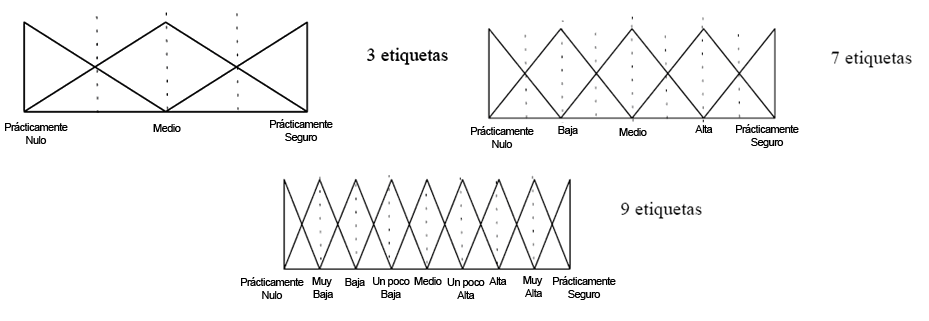
\includegraphics[scale=0.45]{./Imagenes/Etiquetas1.png}
	\caption{Etiquetas triangulares en tres escalas distintas}
	\label{fig:Etiquetas1}
\end{figure}

\section{El modelo de 2-tuplas}

\subsection{Representaci�n con 2-tuplas}
Este modelo de representaci�n de informaci�n ling��stica denominado \emph{2-tuplas} fue introducido por Francisco Herrera y Luis Mart�nez en su art�culo \emph{A 2-tuple fuzzy linguistic representation model for computing with words}\cite{tuplasHerrera}. Est� basado en el modelo simb�lico y toma como base el concepto de \emph{Traducci�n Simb�lica}. La informaci�n se representa mediante una 2-tupla $(p,\alpha)$, donde $p$ es un t�rmino ling��stico y $\alpha$ es un valor num�rico que apoya al valor de la traducci�n simb�lica.

El primer paso para la representaci�n del informaci�n ling��stica es generar un conjunto de t�rminos ling��sticos que podamos usar para expresar informaci�n. Una opci�n para generar este conjunto es suministrar una gram�tica de contexto libre. En cualquier caso, este enfoque implica establecer previamente los conjuntos borrosos asociados con cada t�rmino, y las reglas sem�nticas que los modifican, y esto no es tarea sencilla. 

Otra alternativa consiste en proveer directamente el conjunto de t�rminos en el que consideramos todos los t�rminos distribuidos en una escala y sobre el cual se define un orden total. Por ejemplo, un conjunto $P$ de siete t�rminos podr�a darse as�:

\begin{multline*}	 
	P=\{p_{0}=\ lo\ peor,\ p_{1}=muy\ malo,\ p_{2}=malo,\ p_{3}=medio,\\ 
	\ p_{4}=bueno,\ p_{6}=muy\ bueno,\ p_{7}=lo\ mejor\}
\end{multline*}

En este proyecto utilizaremos etiquetas con pertenencia triangular (Figura \ref{fig:etiquetas2} para simplificar los c�lculos matem�ticos. Por ejemplo, podemos asignar la siguiente sem�ntica (Tabla \ref{tab:semanticaEtiquetas}) a un conjunto de siete t�rminos parecido al definido anteriormente.

\begin{figure}[ht]
	\centering
		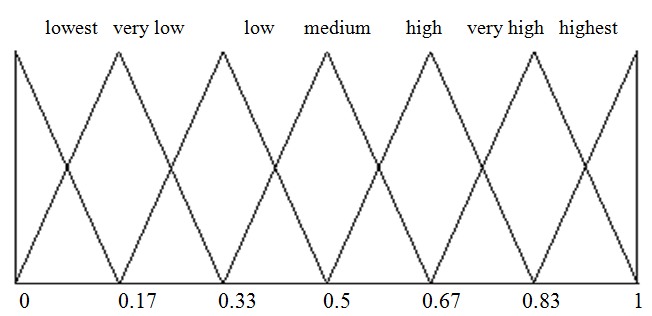
\includegraphics[scale=0.35]{./Imagenes/Etiquetas2.png}
		\caption{Representaci�n de las etiquetas ling��sticas}
		\label{fig:etiquetas2}
\end{figure}

\begin{table}[ht]
	\centering
		\begin{tabular}{ c c }
		\toprule
		\textbf{Etiqueta} & \textbf{Sem�ntica} \\ 
		\midrule
		 Lo m�s alto	& 0.83, 1, 1 \\	
		 Muy alto			& 0.67, 0.83, 1 \\	
		 Alto					& 0.5, 0.67, 0.83 \\	
		 Medio				& 0.33, 0.5, 0.67 \\	
		 Bajo					& 0.17, 0.33, 0.5 \\	
		 Muy bajo			& 0, 0.17, 0.33 \\	
		 Lo m�s bajo	& 0, 0, 0.17 \\	
		 \bottomrule
		\end{tabular}
	\caption{Sem�ntica de las Etiquetas}
	\label{tab:semanticaEtiquetas}
\end{table}

La traducci�n simb�lica de un t�rmino ling��stico $p_{i}\in\left\{ p_{0}, p_{1}, \ldots, p_{g}\right\}$ es un valor num�rico perteneciente al intervalo $\left[-0.5, 0.5\right]$ que representa la \emph{diferencia de informaci�n} entre un c�lculo de la informaci�n $\beta$ evaluado en $\left[0,g\right]$, obtenido despu�s de una operaci�n de agregaci�n simb�lica (que act�a sobre el �ndice de las etiquetas), y el valor m�s cercano en $\left\{0,\ldots,g\right\}$ que indica el �ndice del t�rmino ling��stico m�s cercano en $P\left(p_{i}\right)$.

A partir de este concepto, Herrera y Mart�nez\cite{tuplasHerrera} desarrollan un modelo de representaci�n de informaci�n ling��stica por medio de 2-tuplas $\left(p_{i}, \alpha_{i}\right), p_{i}\in P \text{ y } \alpha_{i} \in \left[-0.5,0.5\right]$, donde $p_{i}$ representa la etiqueta ling��stica central de la informaci�n, y $\alpha_{i}$ es un valor num�rico que representa el desplazamiento del resultado original $\beta$ 	al �ndice de la etiqueta ling��stica m�s cercana en el conjunto de t�rminos, es decir, la Traducci�n Simb�lica.

Este modelo de representaci�n ling��stica define un conjunto de funciones para hacer transformaciones entre t�rminos ling��sticos, 2-tuplas y valores num�ricos.
\begin{defi}
	Sea $p_{i} \in P$ un t�rmino ling��stico, entonces su 2-tupla equivalente viene dada por la funci�n $\theta$ de este modo:
	\begin{equation}	
	\label{eq:theta}
		\begin{gathered}
			\theta:P \rightarrow \left( P\times \left[-0.5,0.5\right)\right) \\
			\theta\left(p_{i}\right)=\left(p_{i},0\right)/p_{i} \in S
		\end{gathered}
	\end{equation}
	\label{def:theta}
\end{defi}

\begin{defi}
	Sea $P=\left\{p_{0}, p_{1},\ldots,p_{g}\right\}$ un conjunto de t�rminos ling��sticos y sea $\beta\in\left[0,g\right]$ un valor que representa el resultado de una operaci�n de agregaci�n simb�lica. Entonces la 2-tupla que representa la informaci�n equivalente a $\beta$ se obtiene con la siguiente funci�n
	
	\begin{equation}
	\label{eq:delta}	
	\begin{gathered}
		\Delta:\left[0,g\right] \rightarrow P\times\left(\left[-0.5,0.5\right)\right) \\
		\Delta\left(\beta\right) = \begin{cases}
			p_{i} & i=round\left(\beta\right)  \\
			\alpha = \beta - i	& \alpha \in \left[ -0.5, 0.5\right)
		\end{cases}		
	\end{gathered}
	\end{equation}
	Donde ``round'' es la operaci�n de redondeo, $p_{i}$ es la etiqueta ling��stica m�s cercana al valor de $\beta$ y $\alpha$ es el valor de la traducci�n simb�lica. 
\label{def:delta}
\end{defi}

\begin{defi}
Sea $P=\left\{p_{0}, p_{1},\ldots,p_{g}\right\}$ un conjunto de t�rminos ling��sticos, y sea $(p_{i}, \alpha_{i})$ una 2-tupla ling��stica. Hay siempre una funci�n $\Delta^{-1}$ tal que, a partir de una 2-tupla, devuelve su valor num�rico equivalente $\beta \in [0,g]$.
\begin{equation}
	\label{eq:deltaInv}
	\begin{gathered}
		\Delta^{-1}:P \times [-0.5,0.5) \rightarrow [0,g]	\\
		\Delta^{-1}(p_{i},\alpha) = i + \alpha = \beta
	\end{gathered}
\end{equation}
\label{def:deltaInv}
\end{defi}

De acuerdo con lo anterior, la representaci�n mediante 2-tuplas ling��sticas presenta ventajas sustantivas respecto a otras metodolog�as, debido a las posibilidades que ofrece para el tratamiento de informaci�n suministrada en distintos dominios de expresi�n, es decir, para operar con informaci�n ling��stica multigranular sin p�rdida de informaci�n.

\section{Jerarqu�as ling��sticas}
El modelo de 2-tuplas parte de contextos ling��sticos con diferentes granularidades, denominados jerarqu�as ling��sticas, las cuales cumplen una serie de reglas y condiciones que permiten unificar la informaci�n en un �nico domino de expresi�n sin p�rdida de informaci�n. Las jerarqu�as ling��sticas est�n compuestas por un conjunto de niveles, donde cada nivel es un conjunto de t�rminos ling��sticos con distinta granularidad al resto de niveles de su jerarqu�a. Cada nivel de una jerarqu�a se puede escribir como: $$L(t,n(t))$$ donde $t$ es el n�mero que indica el nivel de la jerarqu�a y $n(t)$ la granularidad del conjunto ling��stico del nivel $t$.

Los niveles dentro de una jerarqu�a est�n ordenados de acuerdo con su granularidad, es decir, para dos niveles sucesivos $t$ y $t+1$ se cumple que $n(t +1)>n(t)$.

De acuerdo con lo anterior se puede definir una jerarqu�a ling��stica $(LH)$ como la uni�n de todos los niveles 

\begin{equation}
	LH = \bigcup_{t}\ l(t,n(t))
	\label{eq:jerarquiaLinguistica}
\end{equation}

Para analizar la construcci�n de una jerarqu�a ling��stica, teniendo en cuenta que su orden jer�rquico viene dado por el incremento de la granularidad de los conjuntos de t�rminos ling��sticos en cada nivel, se parte de un conjunto de etiquetas S sobre el dominio U en el nivel t, tal:
\begin{equation}
\label{eq:nivelJerarquia}
S=\{s_{0},s_{1}\ldots,s_{n(t)-1}\}
\end{equation}

Siendo $s_{k}$ los t�rminos ling��sticos del conjunto $S$ con $k = 0,\ldots, n(t)$.

Para construir una jerarqu�a ling��stica se puede extender la definici�n de $S$, permitiendo la existencia de varios conjuntos de t�rminos ling��sticos, cada uno con una granularidad distinta en cada nivel. Para ello se introduce el par�metro $n(t)$ en la definici�n de un conjunto de etiquetas, que representa la granularidad del conjunto del nivel $t$ donde est� definido:
\begin{equation}
	S^{n(t)} = \{s_{0}^{n(t)},\ldots, s^{n(t)}_{n(t)-1}\}
\label{eq:conjuntoJerarquia}
\end{equation}
 
En general, cabe admitir que el conjunto de t�rminos del nivel $t+1$ se obtiene de su predecesor como sigue:
\begin{equation}
	L(t,\ n(t)) \rightarrow L(t+1,\ 2\cdot n (t)-1)
\label{eq:nivelesJerarquia}
\end{equation}

Asimismo, existe una funci�n que permite trasladar informaci�n ling��stica de un conjunto de t�rminos a otro sin perdida de informaci�n.Esta funci�n es recursiva y permite la transformaci�n de un termino del nivel $t$ a uno del nivel $t'=t+a$ , con $a \in Z$.

Por comodidad, en el presente trabajo utilizaremos la forma no recursiva de dicha funci�n, que se define as�:
\begin{equation}
	\label{eq:transformarJerarquia}
	\begin{gathered}
		TF^{t}_{t'}: l(t,n(t)) \rightarrow l(t',n(t')) \\
		TF^{t}_{t'}(s_{i}^{n(t)},\alpha^{n(t)}) = \Delta\left(\frac{\Delta^{-1}(s^{n(t)}_{i}, \alpha^{n(t)})\cdot(n(t')-1)}{n(t)-1}\right)
	\end{gathered}
\end{equation}

Esta funci�n es idempotente, esto garantiza la transformaci�n sin p�rdida de informaci�n, por lo que la representaci�n basada en 2-tuplas ling��sticas permite ``traducir'' los resultados de los dominios iniciales de cada experto, con independencia del dominio elegido para el proceso de unificaci�n. 

\section{Resumen}
En este cap�tulo hemos introducido el concepto de computaci�n con palabras.

En primer lugar hemos hecho una breve introducci�n a la l�gica difusa y los conjuntos borrosos, que son la base para definir el concepto de etiqueta ling��stica.

Despu�s hemos introducido el modelo de 2-tuplas para computaci�n con palabras, que nos da las herramientas matem�ticas para computar a partir de t�rminos expresados en lenguaje natural.

Por �ltimo hemos mostrado una manera de trasladar informaci�n ling��stica de un dominio a otro, lo que nos permitir� trabajar con informaci�n estandarizada en el mismo dominio.

En el pr�ximo cap�tulo introduciremos los conceptos de \emph{agregaci�n} y \emph{mayor�a ling��stica}, de forma que, usando el modelo de 2-tuplas mostrado en �ste cap�tulo, podamos recabar una serie de valores de informaci�n cuantitativa y obtener un �nico valor representativo de todos ellos.
\chapter{Agregaci�n de informaci�n ling��sitica}
\section{Introducci�n}
Hasta ahora hemos visto la importancia de la informaci�n ling��stica en el proceso de valoraci�n de empresas, hemos introducido la computaci�n con palabras y el modelo matem�tico de 2-tuplas que nos permite expresar formalmente dicha informaci�n. En el presente cap�tulo veremos c�mo tener en cuenta dicha informaci�n ling��stica, obteniendo un valor representativo que podamos usar en los calculos para la valoraci�n de empresas.

Introduciremos dos m�todos para este fin. Primero introduciremos el operador de mayor�a ling��stica $LAMA$, que ser� el principal objeto de estudio de este trabajo al aplicarlo al proceso de valoraci�n de empresas. Despu�s introduciremos el m�todo de \emph{los expertones}, cuyo impacto en la valoraci�n de empresas ya ha sido estudiado en trabajos anteriores, como por ejemplo los llevados a cabo por Cristina Menda�a Cuervo y otros\cite{TuplasMenda}, y que usaremos en el presente trabajo con fines comparativos.

\section{Agregaci�n mediante mayor�a ling��stica}

Veremos a continuaci�n c�mo funcionan las funciones de agregaci�n de informaci�n ling��stica. Introduciremos en primer lugar el concepto de mayor�a ling��stica para luego presentar el operador de agregaci�n $LAMA$, y su extensi�n $LAMA^{e}$, que permite trabajar con informaci�n ling��stica representada usando el modelo de 2-tuplas.

\subsection{El concepto de Mayor�a ling��stica}

Tradicionalmente el concepto de mayor�a ha estado muy ligado a la idea del grupo mayoritario o a la idea de la mitad m�s uno. Todo esto dio lugar a las denominadas \emph{dictaduras de la mayor�a}, donde se hac�a lo que indicada el grupo m�s numeroso sin tener en cuenta a los grupos minoritarios. En contra de est�s actitudes surgieron nuevas formas o  m�todos  de decisi�n que intentaban solucionar estos problemas, y con ellas las herramientas necesarias para llevarlas a cabo, pero cual ha sido la sorpresa que al analizar dichos m�todos se ha podido comprobar que las dictaduras de la mayor�as han dado lugar a las dictaduras de las minor�as, donde las opiniones minoritarias son m�s influyentes que las opiniones mayoritarias.

Este problema se muestra en el siguiente ejemplo: sean los siguientes elementos: $\left\{0.7, 0.7, 0.7, 0.7, 0.5, 0.4, 0.1, 0.1, 0.1\right\}$. Si se analiza este ejemplo se puede apreciar que el $55\%$ de los elementos es mayor que 0.4, siendo el valor 0.7 el 44\% del total. Debido a este resultado, se puede suponer que un valor que fuese representativo del grupo, deber�a ser mayor a 0.5 e inferior a 0.7. Sin embargo, si se obtiene un valor de representaci�n para dichos valores haciendo uso de los operadores tradicionales m�s utilizados como son la media aritm�tica y media geom�trica, se obtendr�an los valores 0.444 y 0.331 respectivamente, valores que aun siendo correctos desde un punto de vista matem�tico, sem�nticamente no reflejan la opini�n mayoritaria y s� el valor de la minor�a. 

Otro ejemplo que muestra el problema anterior es el siguiente: Supongamos un pueblo donde residen 1001 personas, las cuales tienen los siguientes ingresos mensuales: 1.000 personas tienen unos ingresos de 1000 euros, mientras que 1 persona tiene unos ingresos de 1000.000.000 euros. Si se calculan los ingresos medios, y nuevamente se utiliza la media aritm�tica resulta que dicho pueblo muestra que sus habitantes tienen unos ingresos medios mensuales de 1.000.000 de euros aproximadamente. Nuevamente aun siendo correcto este valor desde un punto de vista matem�tico, sin embargo desde un punto de vista sem�ntico y de informaci�n social dicho valor dista mucho de dar una informaci�n que sea representativa de la mayor�a de la poblaci�n. 

Con objeto de paliar los problemas anteriores, ha surgido un nuevo concepto denominado Mayor�a, que trata de obtener un valor de opini�n que sea representativo de la mayor�a pero sin olvidar a las minor�as. 

La diferencia entre los procesos cl�sicos y los nuevos procesos denominados de mayor�a, se basa en la forma en que son considerados los elementos a la hora de obtener un valor de representaci�n. Como muestra la figura \ref{fig:procesos1}, en los procesos cl�sicos los elementos son considerados de manera aislada, y sobre estos elementos se opera para obtener un valor para el grupo. Sin embargo, en los procesos de mayor�a los elementos no son considerados de manera individual si no que forman grupos de elementos, en base a una funci�n de distancia entre ellos, que comparten una misma opini�n y que se enfrentan unos con otros para obtener un valor com�n. 

El enfrentamiento entre elementos de distintos grupos se lleva a cabo tomando un elemento de cada uno de los grupos, con los cuales se opera para obtener un nuevo valor que sea representante de los mismos. La operaci�n se puede llevar a cabo mediante operadores tradicionales. Los elementos que han sido considerados son eliminados de los grupos iniciales, pasando a formar un nuevo grupo con valor igual al calculado y cardinalidad el n�mero de elementos que han sido considerados. Este proceso continua hasta que queda un solo grupo de elementos. Aquellos grupos que en un momento dado han enfrentado a todos sus representantes, dejan de participar en el proceso y por lo tanto de influir a partir de ese momento en el valor final. 

\begin{figure}
	\centering
		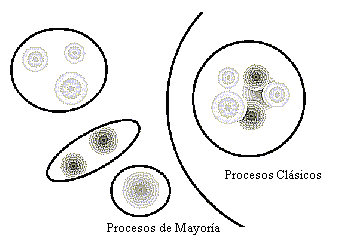
\includegraphics[scale=0.6]{Imagenes/Procesos1.png}
	\caption{Procesos de Mayor�a y Procesos Cl�sicos.}
	\label{fig:procesos1}
\end{figure}

Actualmente el concepto anterior que ha sido definido como Mayor�a, ha dado lugar al concepto de Mayor�a Fuzzy. La Mayor�a Fuzzy se modela a trav�s del uso de cuantificadores ling��sticos, tales como ``al menos el 80\%'', ``muchos'', ``algunos'', etc�tera, defini�ndose formalmente como un subconjunto borroso dentro de un dominio num�rico, que trata de delimitar el n�mero de elementos de cada uno de los grupos. 

La sem�ntica de un subconjunto borroso se describe a trav�s del uso de una funci�n de pertenencia la cual describe la compatibilidad de un valor absoluto o porcentual con respecto al concepto expresado por el cuantificador ling��stico. De esta forma, el cuantificador ling��stico se puede ver como un concepto borroso que se refiere a la cantidad de elementos a considerar en el conjunto de referencia. En la ecuaci�n \ref{eq:muchos} vemos la definici�n matem�tica del cuantificador ling��stico muchos, y en la figura \ref{fig:graficaMuchos} su representaci�n gr�fica.

\begin{align}
\mu_{muchos}(x) = 
\begin{cases}	
	1 & x \geq 0.9 \\
	2x-0.8 &	0.4 \leq x <0.9	\\
	0	&	x \leq 0.4 	
\end{cases}
\label{eq:muchos}
\end{align}

\begin{figure}[ht]
	\centering
		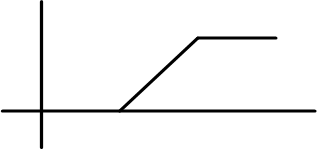
\includegraphics[scale=0.4]{Imagenes/GraficaMuchos.png}
	\label{fig:graficaMuchos}
	\caption{Cuantificador ``muchos''}
\end{figure}

La aplicaci�n del cuantificador se puede llevar a cabo atendiendo a aspectos sociales, dando lugar a la cuantificaci�n individual o en grupo.

La  cuantificaci�n individual consiste en indicar el grado con que cada miembro del conjunto de valores representa el concepto de mayor�a. Para ello, esta estrategia aplica la sem�ntica del cuantificador directamente sobre el peso individual de cada elemento de la agregaci�n, donde el peso ha sido previamente calculado con un operador de agregaci�n. La figura \ref{fig:cuantificadorIndividual} muestra un ejemplo de aplicaci�n de la cuantificaci�n individual sobre un conjunto de valores a agregar. Los valores por encima de la l�nea no son considerados en la agregaci�n.

\begin{figure}[ht]
	\centering
		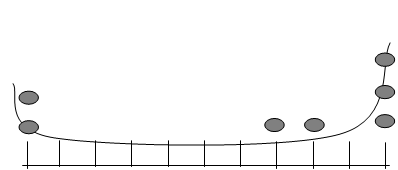
\includegraphics[scale=0.6]{Imagenes/CuantificadorIndividual.png}
	\label{fig:cuantificadorIndividual}
	\caption{Representaci�n gr�fica del corte del cuantificador con la sem�ntica de cuantificaci�n individual}
\end{figure}

Pero desde un punto de vista social existen problemas de toma de decisi�n en grupo donde se debe cumplir la premisa, que todos los grupos de opiniones est�n representados por al menos un representante. Como muestra la figura \ref{fig:cuantificadorIndividual} esta premisa no siempre se cumple con la cuantificaci�n individual ya que existen grupos de opini�n que son eliminados del proceso de decisi�n. Para solucionar este problema se propone la cuantificaci�n en grupo, la cual siempre garantiza dicha premisa. La figura \ref{fig:cuantificadorGrupo} muestra un ejemplo de aplicaci�n de la cuantificaci�n en grupo sobre un conjunto de valores a agregar. Los valores por encima de la l�nea no son considerados en la agregaci�n.

\begin{figure}[ht]
	\centering
		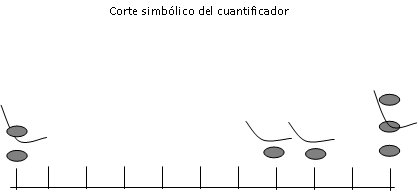
\includegraphics[scale=0.6]{Imagenes/CuantificadorGrupo.png}
		\label{fig:cuantificadorGrupo}
		\caption{Representaci�n gr�fica del corte del cuantificador con la sem�ntica de cuantificaci�n en grupo}
\end{figure}

La aplicaci�n de los procesos de mayor�a fuzzy permite dar mayor representatividad a los resultados en los procesos de decisi�n, permitiendo modelar conceptos como muchos, pocos, algunos, etc. En la figura \ref{fig:dominios} se muestra el dominio de los procesos cl�sicos, los procesos de mayor�a  y los procesos de mayor�a fuzzy. Para ello se ha considerado un ejemplo con 7 valores que han sido representados mediante elipses. 
\begin{figure}[ht]
	\centering
			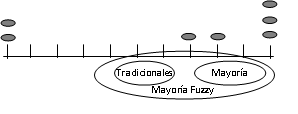
\includegraphics{Imagenes/Dominios.png}
		\label{fig:dominios}
	\caption{Dominio de los procesos de decisi�n tradicionales, de mayor�a, y de mayor�a \emph{fuzzy}}
\end{figure}

Diferentes operadores de mayor�a han sido definidos en la literatura. As�, para representar el concepto de mayor�a en entornos aditivos, destaca el operador $MA-OWA$, o para mayor�a cuantificada operadores como $IOWA$ y $QMA-OWA$. A continuaci�n se va a presentar de manera formal el operador $LAMA$, que ser� utilizado posteriormente para agregar la informaci�n ling��stica al proceso de valoraci�n de empresas. 

\subsection{Operadores de mayor�a ling��sticos aditivos. El operador $LAMA$}

El operador $LAMA$, acr�nimo de \emph{Linguistic Aggregation of Majority Additive} o \emph{Agregaci�n linguistica de mayor�a aditiva} es presentado en el art�culo \emph{LAMA: A linguistic aggregation of Majority Additive Operator}\cite{PelaezLAMA} de J.I. Pel�ez y J.M. Do�a, y es un operador de mayor�a para entornos ling��sticos con un espacio de etiquetas $S$, que se define como una media aritm�tica de medias aritm�ticas, de forma que el resultado final es una media aritm�tica ponderada.

\begin{defi}
\label{def:lama}
Sean las etiquetas $p_{1}, p_{2}, \ldots, p_{n} \in  P$ tales que $t > 0$ y sea $\delta_{1},\delta_{2},\ldots,\delta_{n} \in N$ las frecuencias o cardinalidad de las etiquetas, donde $\delta_{i}\leq\delta_{i+1}$ para todo $1\leq i \leq n-1 $. El operador $LAMA$ es la etiqueta $p_{m}$ dada por:
\begin{gather*}
p_{m} = LAMA((p_{1},\delta_{1}),(p_{2},\delta_{2}),\ldots,(p_{n},\delta_{n}))	\\
= p_{1} \otimes \lambda_{1} \oplus p_{2} \otimes \lambda_{2} \oplus \ldots \oplus p_{n} \otimes \lambda_{n}
\end{gather*}
donde
	\begin{align*}
	\lambda_{i} = 
		\begin{cases}
		\frac{1}{d_{1}}																																									&	\text{si } i=1	\\
		\frac{1}{d_{1}} \cdot \frac{1-n^{\delta_{2}}}{1-n}																							&	\text{si }	i=2	\\
		\lambda_{i-1} + \frac{1}{d_{i-1}} \cdot \frac{1-(n-i+2)^{\delta_{i} - \delta_{i-1}}}{1-(n-i+2)}	& \text{si } i > 2	\\
		\end{cases}	
	\end{align*}
con
	\begin{align*}
	d_{i} = 
		\begin{cases}
			1																																					&	\text{si } i=1, n=1	\\
			n^{\delta_{2}}																														&	\text{si } i=1, n=2 \\
			n^{\delta_{2}} \cdot \prod\limits^{n-2}_{j=1}{(n-j)^{\delta_{j+1}-\delta_{j+1}}}	& \text{si } i=1, n>2 \\
			\prod\limits^{n-2}_{j=i-1}{(n-j)^{\delta_{j+1}-\delta_{j+1}}}										& \text{si } i>1
		\end{cases}
	\end{align*}
y donde $\oplus$ es la suma de etiquetas y $\otimes$ es el producto de una etiqueta por un real positivo.
\end{defi}

\subsection{El operador $LAMA$ utilizando representaci�n con 2-tuplas}
Podemos definir el operador $LAMA^{e}$ como una extensi�n del operador $LAMA$ para operar con informaci�n ling��stica representada mediante el modelo de 2-tuplas expuesto.

\begin{defi}
\label{def:lamae}
Sean $(p_{1}, \alpha_{1}),\ (p_{2},\alpha_{2}),\ldots,\ (p_{n}, \alpha_{n})$ las 2-tuplas a ser agregadas, y sean$ \delta_{1},\ \delta_{2},\ldots\ \delta_{n} \in N$ la frecuencia o cardinalidad de dichas 2-tuplas, donde $\delta_{i} \leq \delta_{i+1}$ para todo $1 \leq i \leq n-1$. El operador $LAMA^{e}$ es la 2-tupla $(p_{m},\alpha_{m})$ dada por:

\begin{equation}
\begin{split}
LAMA^{e}((p_{1}, \alpha_{1}),\ (p_{2},\alpha_{2}),\ldots,\ (p_{n}, \alpha_{n})) = \Delta(\Delta^{-1}(p_{1},\alpha{1})\cdot w_{1} \\
+ \Delta^{-1}(p_{2},\alpha_{2})\cdot w_{2} + \ldots + \Delta^{-1}(p_{n},\alpha_{n})\cdot w_{n})
\end{split}
\label{eq:lamae}
\end{equation}

donde $w_i\in[0,1]$ y $\sum\limits_{i=1}^{n}{w_i} = 1$.

El valor de cada peso $w_{i}$ se calcula a partir de las cardinalidades de cada 2-tupla de la siguiente manera.

Sea $\delta_i$ la cardinalidad de la etiqueta $i$ con $\delta_i>0$, entonces:

\begin{equation}
\begin{split}
w_i=  &\frac{\gamma_i^{\delta_{min}}}{\Theta_{\delta_{max}}\cdot\Theta_{\delta_{max}-1}\cdot\dots\cdot\Theta_{\delta_{min}-1}\cdot\Theta_{\delta_{min}}} + 
\frac{\gamma_i^{\delta_{min}}}{\Theta_{\delta_{max}}\cdot\Theta_{\delta_{max}-1}\cdot\dots\cdot\Theta_{\delta_{min}-1}} + \\ 
& \cdots +
\frac{\gamma_i^{\delta_{min}}}{\Theta_{\delta_{max}}\cdot\Theta_{\delta_{max}-1}} +
\frac{\gamma_i^{\delta_{min}}}{\Theta_{\delta_{max}}}
\end{split} 
\label{eq:weights}
\end{equation}

donde
\begin{equation}
	\gamma_i^k = 
		\begin{cases}
		1 & if \  \delta_i \geq k \\
		0 & en\ otro\ caso
		\end{cases}
	\label{eq:gammaForWeights}
\end{equation}

y

\begin{equation}
	\Theta_i = 
		\begin{cases}
			(numero\ de\ etiqueta\ con\ cardinalidad \geq i) + 1 & si\ i \neq \delta_{min} \\
			(numero\ de\ etiqueta\ con\ cardinalidad \geq i) 		 & en\ otro\ caso
		\end{cases}	
\label{eq:thetaForWeights}
\end{equation}	
\end{defi}


El valor de la cardinalidad de cada 2-tupla puede calcularse usando dos metodolog�as diferentes:
\begin{enumerate}
    \item Usando como cardinalidad el n�mero de 2-tuplas que representan la misma informaci�n
	\item Usando como cardinalidad el n�mero de 2-tuplas que representan informaci�n similar. 
\end{enumerate}
\begin{defi}
\label{def:comparacion2tupla}
Sean $(p_{i},\alpha_{1})$ y $(p_{j},\alpha_{2})$ dos 2-tuplas, cada una representando una cantidad de informaci�n, entonces, si $i=j$, entonces:
\begin{itemize}
	\item Si $\alpha_{1} = \alpha_{2}$, entonces ambas tuplas representan la misma informaci�n
	\item En otro caso, las tuplas representan informaci�n similar, donde:
	\begin{itemize}
		\item Si $\alpha_{1} < \alpha_{2}$, entonces $(p_{i},\alpha_{1})$ es menor que $(p_{j},\alpha_{2})$
		\item Si $\alpha_{1} > \alpha_{2}$, entonces $(p_{i},\alpha_{1})$ es mayor que $(p_{j},\alpha_{2})$
	\end{itemize}
\end{itemize}   
\end{defi}

\section{M�todo de los expertones}

Definidos por Kaufmann\cite{expertonesKaufmann}, el m�todo de los expertones permite agregar la opini�n de varios expertos a partir de valoraciones dadas por ellos, llevando una estad�stica de todos los valores posibles, que depender� de la escala usada. Esta estad�stica se somete a un proceso de estandarizaci�n de acuerdo con el n�mero de opiniones disponible. Concretamente, la funci�n complementaria de probabilidad acumulada es lo que llamamos expert�n. 

Aplicado al modelo de 2-tuplas, lo que haremos ser� recoger las opiniones de los distintos expertos, normalizadas a un �nico conjunto de etiquetas, y a partir de la frecuencia absoluta de cada etiqueta, calcularemos su funcion de probabilidad acumulada complementaria.

No es objetivo de este trabajo presentar la teor�a completa sobre los expertones, por lo que simplemente ilustraremos su uso con un ejemplo pr�ctico para ajustar un intervalo sobre un expertizaje expresado con el modelo de 2-tuplas. 

\begin{ejem}
Consideremos el intervalo $[0'04, 0'05]$ de posibles tipos de interes inicial para la valoraci�n de una empresa.

Para alcanzar un consenso sobre la validez de dicha informaci�n, se pide a diez expertos que den su opinion, usando distintos conjuntos de etiquetas sem�nticas. Tomando como conjunto de referencia el conjunto $S_{9}$, obtenemos las opiniones reflejadas en la tabla \ref{tab:opinionExpertones}
\begin{table}[!htb]
	\centering
		\begin{tabular}{c c}
			\toprule
			Experto	&	$[0'04, 0'05]$	\\	
			\midrule
			$e_{1}$	&	$(S_{6}^{9},0) - (S_{8}^{9}, 0)$	\\	
			$e_{2}$	&	$(S_{5}^{9},0'33) - (S_{7}^{9}, -0'33)$	\\	
			$e_{3}$	&	$(S_{6}^{9},0)$	\\	
			$e_{4}$	&	$(S_{5}^{9},0)$	\\	
			$e_{5}$	&	$(S_{6}^{9},0) - (S_{8}^{9}, 0)$	\\	
			$e_{6}$	&	$(S_{8}^{9},0)$	\\	
			$e_{7}$	&	$(S_{8}^{9},0)$	\\	
			$e_{8}$	&	$(S_{5}^{9},0) - (S_{7}^{9}, 0)$	\\	
			$e_{9}$	&	$(S_{8}^{9},0)$	\\	
			$e_{10}$	&	$(S_{0}^{9},0) - (S_{1}^{9}, 0)$	\\
			\bottomrule			
		\end{tabular}
	\caption{Opinion de los expertos}
	\label{tab:opinionExpertones}
\end{table}

Observamos las frecuencias de cada 2-tupla. Para estandarizar los valores, dividimos por 10, que es el n�mero de opiniones disponibles, obteniendo as� la tabla \ref{tab:cardinalidades}

\begin{table}[!htb]
		\centering
		\begin{tabular} {c | c c | c c}
			\toprule
			\multicolumn{1}{c}{2-tupla} & \multicolumn{2}{c}{$[0'04, 0'05]$} & $p(0'4)$	& $p (0'5)$ \\
			\midrule
			$(S_{8}^{9},0)$	&	3	&	5 & 0'3	& 0'5	\\
			$(S_{7}^{9},0)$	&	0	&	1	& 0	& 0'1	\\
			$(S_{7}^{9},-0'33)$	&	0	&	1	& 0	& 0'1	\\
			$(S_{6}^{9},0)$	&	3	&	1	& 0'3	& 0'1	\\
			$(S_{5}^{9},0'33)$	&	1	&	0	& 0'1	& 0	\\
			$(S_{5}^{9},0)$	&	2	&	1	& 0'2	& 0'1	\\				
			$(S_{1}^{9},0)$	&	0	&	1	& 0	& 0'1	\\
			$(S_{0}^{9},0)$	&	1	& 0 & 0'1	& 0	\\
			\bottomrule
		\end{tabular}
	\caption{Cardinalidades y probabilidades}
	\label{tab:cardinalidades}
\end{table}

Ahora, ordenando las tuplas de ``menor'' a ``mayor'', incluyendo los nueve valores del conjunto sem�ntico utilizado, aplicamos la funci�n acumulada complementaria para obtener el \emph{expert�n} reflejado en la tabla \ref{tab:experton}.

\begin{table}[!htb]
		\centering
		\begin{tabular} {c | c c }
			\toprule
			\multicolumn{3}{c}{$[0.04, 0.05]$} \\
			\midrule
			$(S_{0}^{9},0)$			&	0.9	& 1	\\
			$(S_{1}^{9},0)$			&	0.9	&	0.9	\\
			$(S_{2}^{9},0)$			&	0.9	&	0.9	\\
			$(S_{3}^{9},0)$			&	0.9	&	0.9	\\
			$(S_{4}^{9},0)$			&	0.9	&	0.9	\\
			$(S_{5}^{9},0)$			&	0.7	&	0.8	\\
			$(S_{5}^{9},0'33)$	&	0.6	&	0.8	\\
			$(S_{6}^{9},0)$			&	0.3	&	0.7	\\
			$(S_{7}^{9},-0'33)$	&	0.3	&	0.6	\\
			$(S_{7}^{9},0)$			&	0.3	&	0.5	\\
			$(S_{8}^{9},0)$			&	0		&	0	\\					
			\bottomrule
		\end{tabular}
	\caption{Expert�n para el intervalo $[0.04, 0.05]$}
	\label{tab:experton}
\end{table}

Para obtener el $R^{+}$-experton para el intervalo $[\alpha_{0},\alpha_{1}]$ aplicamos
	\[
	\alpha_{0}+\left(\left(\alpha_ {1}-\alpha_{0}\right)\right)\cdot Experton
	\]

De esta forma obtenemos el $R^{+}$-Experton para el ejemplo en la tabla \ref{tab:rExperton}.
\begin{table}[!htb]
		\centering
		\begin{tabular} {c | c c | c c }
			\toprule
			\multicolumn{5}{c}{$[0.04, 0.05]$} \\
			\midrule
			&\multicolumn{2}{c}{$Experton$}&\multicolumn{2}{c}{$R^{+}$-Experton} \\
			\midrule
			$(S_{0}^{9},0)$			&	0.9	& 1 	& 0.049 & 0.010 \\
			$(S_{1}^{9},0)$			&	0.9	&	0.9	& 0.049 & 0.050 \\
			$(S_{2}^{9},0)$			&	0.9	&	0.9	& 0.049	& 0.049 \\
			$(S_{3}^{9},0)$			&	0.9	&	0.9	& 0.049	& 0.049 \\
			$(S_{4}^{9},0)$			&	0.9	&	0.9	& 0.049	& 0.049 \\
			$(S_{5}^{9},0)$			&	0.7	&	0.8	& 0.049	& 0.049 \\
			$(S_{5}^{9},0'33)$	&	0.6	&	0.8	& 0.047	& 0.048 \\
			$(S_{6}^{9},0)$			&	0.3	&	0.7	& 0.043	& 0.047 \\
			$(S_{7}^{9},-0'33)$	&	0.3	&	0.6	& 0.043	& 0.046 \\
			$(S_{7}^{9},0)$			&	0.3	&	0.5	& 0.043	& 0.045 \\
			$(S_{8}^{9},0)$			&	0		&	0		& 0.040	& 0.040 \\					
			\bottomrule
		\end{tabular}
	\caption{Expert�n y $R^{+}$-Experton para el intervalo $[0.04, 0.05]$}
	\label{tab:rExperton}
\end{table}

Finalmente obtenemos el intervalo ajustado, calculando la esperanza matem�tica del $R^{+}$-expert�n. Esto es, sumando todos los valores del expert�n en cada extremo del intervalo (excepto el nivel 0), y dividiendo entre el n�mero de elementos.
	
	\[
	\begin{gathered}
	i_{inicial} = \left[0,04, 0.05\right] \\
	i_{ajustado} = \left[0.04610, 0.04720\right]
	\end{gathered}
\]

\end{ejem}

\section{Resumen}
En este cap�tulo hemos introducido el concepto de agregaci�n de informaci�n ling��stica mediante el concepto de mayor�a.

Hemos presentado el operador de mayor�a ling��stica $LAMA$ en su forma gen�rica, as� como su extensi�n para trabajar con el modelo de dos tuplas.

As� mismo hemos visto un ejemplo de una metodolog�a alternativa para agregar informaci�n ling��stica a valores cuantitativos usando el m�todo cl�sico de los expertones. 

En el pr�ximo cap�tulo veremos como utilizar estas dos metodolog�as aplicadas al proceso de valoraci�n de una empresa. 
\chapter{Modelos de valoraci�n con mayor�a}
\section{Introducci�n}
Hemos visto hasta ahora los conceptos b�sicos sobre valoraci�n de empresas, as� como varios m�todos para realizar esta valoraci�n.

Hemos introducido tambi�n los fundamentos de l�gica difusa y computaci�n con palabras, as� como el modelo de 2-tuplas, con el que expresar de forma computable la informaci�n cualitativa que queremos a�adir al proceso de valoraci�n.

Finalmente, hemos introducido el concepto de agregaci�n ling��stica, proporcionando herramientas para obtener un valor representativo de dicha informaci�n cualitativa.

En el presente cap�tulo fusionaremos todas las herramientas vistas hasta ahora, aplicando un expertizaje en lenguaje natural al proceso de valoraci�n de una empresa

\section{Metodolog�a}
En el cap�tulo 2 hemos visto las expresiones matem�ticas para la valoraci�n de empresas utilizando tanto el m�todo del \textit{cashflow} como el m�todo mixto de an�lisis operativo. 

En ambos m�todos procederemos de la misma manera: para cada estimaci�n que llevemos a cabo, los expertos consultados expresar�n sus valoraciones dentro de sus propios dominios de expresi�n. Despu�s, mediante el modelo ling��stico de 2-tuplas normalizaremos todas las valoraciones a un �nico dominio, en el cual a�adiremos la informaci�n a cada intervalo num�rico a ser considerado utilizando el operador $LAMA$. Por �ltimo estandarizaremos los resultados obtenidos de acuerdo con el dominio unificado que hayamos elegido inicialmente.

En este punto, para estimar los intereses, los beneficios futuros o la estimaci�n de cashflow, aplicaremos la siguiente expresi�n a cada intervalo:

	\[
	[\left[limite\ inferior\right] + \left(limite\ sup - limite\ inf\right)\cdot\left[L_{1}^{N}, L_{2}^{N}\right]
	\]

Siendo $L_{1}^{N}, L_{2}^{N}$ los valores estandarizados tras aplicar el operador $LAMA$ a las etiquetas ling��sticas.

Una vez obtengamos los valores ajustados para cada intervalo, aplicaremos la expresi�n matem�tica correspondiente a cada m�todo de valoraci�n, tal y como vimos en el cap�tulo 2.

Una vez agregada la informaci�n usando el operador $LAMA$, utilizaremos tambi�n, con fines comparativos, el m�todo de los expertones para obtener una valoraci�n ajustada usando la informaci�n cuantitativa. 

Para ello seguiremos la metodolog�a de c�lculo de expertones que vimos en el ejemplo del cap�tulo anterior, de forma que obtengamos los intervalos ajustados con los que aplicar el m�todo elegido para la valoraci�n.

\section{M�todo mixto con agregaci�n LAMA}

A continuaci�n estudiaremos un ejemplo de agregaci�n de informaci�n ling��stica al proceso de valoraci�n de empresas utilizando el m�todo mixto del an�lisis operativo. 

Para analizar el valor de la empresa, el proceso de estimaci�n para los tipos de inter�s normalmente comienza con un an�lisis que permite considerar los posibles intervalos en los cuales se espera que la tasa de inter�s fluct�e durante los periodos considerados en el estudio, de forma que estos sirvan como punto de inicio en la negociaci�n entre las partes que participan en el proceso de valoraci�n.

\subsection{C�lculo de los intereses futuros}

En el ejemplo pr�ctico que proponemos, se ha establecido un periodo de an�lisis de tres a�os, para los cuales hemos considerado los siguientes intervalos de tasas de inter�s:
\[
	\left[0.04, 0.05\right],\ \left[0.045, 0.06\right],\ \left[0.05, 0.06\right]
\]

Con el objetivo de alcanzar un consenso para la validez de la informaci�n, es posible consultar a varios expertos de forma que validen su conformidad con cada uno de los valores iniciales. La informaci�n requerida, de acuerdo con con las consideraciones expuestas en los anteriores cap�tulos, debe ser expresadas en t�rminos familiares a cada uno de los expertos consultados. Por tanto, se han definido tres conjuntos ling��sticos distintos, con la siguiente sem�ntica:

Conjunto 1: 
\begin{equation*}
	S_{5}=\left\{ 
		S_{4}^{5}\left(MuyAlto\right), 
		S_{3}^{5}\left(Alto\right), 
		S_{2}^{5}\left(Medio\right), 
		S_{1}^{5}\left(Bajo\right), 
		S_{0}^{5}\left(MuyBajo\right)  
	\right\}	
	\label{eq:set1}
\end{equation*}

Conjunto 2: 
\begin{equation*}
	\begin{split}
	S_{7} & = \{
		S_{6}^{7}\left(MuyAlto\right),
		S_{5}^{7}\left(Alto\right),
		S_{4}^{7}\left(LigeramenteAlto\right),
		S_{3}^{7}\left(Medio\right),\\
		& \ S_{2}^{7}\left(LigeramenteBajo\right),
		S_{1}^{7}\left(Bajo\right),
		S_{0}^{7}\left(MuyBajo\right) \}
	\end{split}
	\label{eq:set2}
\end{equation*}

Conjunto 3: 
\begin{equation*}
	\begin{split}
	S_{9} & =\{
		S_{8}^{9}\left(CasiSeguro\right),
		S_{7}^{9}\left(MuyAlto\right),
		S_{6}^{9}\left(Alto\right),
		S_{5}^{9}\left(LigeramenteAlto\right),\\
		&\ S_{4}^{9}\left(Medio\right),
		S_{3}^{9}\left(LigeramenteBajo\right),
		S_{2}^{9}\left(Bajo\right),
		S_{1}^{9}\left(MuyBajo\right),
		S_{0}^{9}\left(CasiNulo\right)		
	\}
	\end{split}	
	\label{eq:set3}
\end{equation*}

De este modo, una vez consultado un conjunto de 10 expertos, obtenemos las valoraciones ling��sticas para cada dominio, reflejadas en la tabla \ref{tab:expertizajeDiferentesDominios}.

\begin{table}[!htb]
	\centering	
	\begin{tabular}{c | c  c  c }
		\toprule
		Experto	& $\left[0.04, 0.05\right]$	& $\left[0.04, 0.05\right]$ & $\left[0.04, 0.05\right]$ \\ 
		\midrule
		$e_{1}$		& $S_{3}^{5} - S_{4}^{5}$		&	$S_{4}^{5}$							&	$S_{1}^{5} - S_{2}^{5}$		\\ 
		$e_{2}$		& $S_{4}^{7} - S_{5}^{7}$		&	$S_{4}^{7} - S_{6}^{7}$	&	$S_{0}^{7}$								\\ 
		$e_{3}$		& $S_{6}^{9}$								&	$S_{8}^{9}$							&	$S_{0}^{9} - S_{3}^{9}$		\\ 
		$e_{4}$		& $S_{5}^{9}$								&	$S_{7}^{9} - S_{8}^{9}$	&	$S_{2}^{9} - S_{4}^{9}$		\\ 
		$e_{5}$		& $S_{3}^{5} - S_{4}^{5}$		&	$S_{3}^{5} - S_{4}^{5}$	&	$S_{1}^{5}$								\\ 
		$e_{6}$		& $S_{4}^{5}$								&	$S_{4}^{5}$							&	$S_{0}^{5} - S_{1}^{5}$		\\ 
		$e_{7}$		& $S_{8}^{9}$								&	$S_{5}^{9} - S_{7}^{9}$	&	$S_{2}^{9} - S_{4}^{9}$		\\ 
		$e_{8}$		& $S_{5}^{9} - S_{7}^{9}$		& $S_{5}^{9} - S_{6}^{9}$	&	$S_{5}^{9} - S_{7}^{9}$		\\ 
		$e_{9}$		& $S_{6}^{7}$								&	$S_{1}^{7} - S_{2}^{7}$	&	$S_{5}^{7} - S_{6}^{7}$		\\ 
		$e_{10}$	& $S_{0}^{9} - S_{1}^{9}$		&	$S_{5}^{9} - S_{6}^{9}$	&	$S_{6}^{9} - S_{8}^{9}$		\\ 
		\bottomrule
	\end{tabular}
	\caption{Valoraciones ling��sticas para cada dominio}
	\label{tab:expertizajeDiferentesDominios}
\end{table}

A continuaci�n ser� necesario proceder a la estandarizaci�n de los valores establecidos por los expertos. Para esto es necesario determinar un conjunto de t�rminos ling��sticos que ser� usado como base para unificar la informaci�n. En este caso, dado que la mayor�a de expertos ha utilizado el dominio $S_{9}$, este ser� el elegido, aunque ser� posible utilizar cualquier otro. 

Aplicando la ecuaci�n \ref{eq:transformarJerarquia}, pasamos todos los valores al dominio $S_{9}$ obteniendo las valoraciones reflejadas en las tablas \ref{tab:expertizajeEstandar1}, \ref{tab:expertizajeEstandar2} y \ref{tab:expertizajeEstandar3}. 

\begin{table}[!htb]
\centering
	\begin{tabular}{c | c }
		\toprule
		Experto	& $\left[0.04, 0.05\right]$	\\ 
		\midrule
		$e_{1}$		& $(S_{6}^{9}, 0)-(S_{8}^{9}, 0)$ 				\\ 
		$e_{2}$		& $(S_{5}^{9}, 0.33)-(S_{7}^{9}, -0.33)$	\\ 
		$e_{3}$		& $(S_{6}^{9}, 0)$												\\ 
		$e_{4}$		& $(S_{5}^{9}, 0)$												\\ 
		$e_{5}$		& $(S_{6}^{9}, 0)-(S_{8}^{9}, 0)$					\\ 
		$e_{6}$		& $(S_{8}^{9}, 0)$												\\ 
		$e_{7}$		& $(S_{8}^{9}, 0)$												\\ 
		$e_{8}$		& $(S_{5}^{9}, 0)-(S_{7}^{9}, 0)$					\\ 
		$e_{9}$		& $(S_{8}^{9}, 0)$												\\ 
		$e_{10}$	& $(S_{0}^{9}, 0)-(S_{1}^{9}, 0)$					\\ 
		\bottomrule
	\end{tabular}
	\caption{Valoraciones ling��sticas estandarizadas - Intervalo 1}
	\label{tab:expertizajeEstandar1}
\end{table}

\begin{table}[!htb]
\centering
	\begin{tabular}{c | c  c  c }
		\toprule
		Experto	& $\left[0.04, 0.05\right]$ \\ 
		\midrule
		$e_{1}$		&	$(S_{8}^{9}, 0)$										\\ 
		$e_{2}$		&	$(S_{5}^{9}, 0.33)-(S_{8}^{9}, 0)$	\\ 
		$e_{3}$		&	$(S_{8}^{9}, 0)$										\\ 
		$e_{4}$		&	$(S_{7}^{9}, 0)-(S_{8}^{9}, 0)$			\\ 
		$e_{5}$		&	$(S_{6}^{9}, 0)-(S_{8}^{9}, 0)$			\\ 
		$e_{6}$		&	$(S_{6}^{9}, 0)$										\\ 
		$e_{7}$		&	$(S_{5}^{9}, 0)-(S_{7}^{9}, 0)$			\\ 
		$e_{8}$		& $(S_{5}^{9}, 0)-(S_{6}^{9}, 0)$			\\ 
		$e_{9}$		&	$(S_{1}^{9}, 0.33)-(S_{3}^{9}, -0.33)$	\\ 
		$e_{10}$	&	$(S_{5}^{9}, 0)-(S_{6}^{9}, 0)$			\\ 
		\bottomrule
	\end{tabular}
	\caption{Valoraciones ling��sticas estandarizadas - Intervalo 2}
	\label{tab:expertizajeEstandar2}
\end{table}

\begin{table}[!htb]
\centering	
	\begin{tabular}{c | c  c  c }
		\toprule
		Experto	& $\left[0.04, 0.05\right]$ \\ 
		\midrule
		$e_{1}$		&	$(S_{2}^{9}, 0)-(S_{4}^{9}, 0)$	\\ 
		$e_{2}$		&	$(S_{0}^{9}, 0)-(S_{4}^{9}, 0)$	\\ 
		$e_{3}$		&	$(S_{0}^{9}, 0)-(S_{3}^{9}, 0)$	\\ 
		$e_{4}$		&	$(S_{2}^{9}, 0)-(S_{4}^{9}, 0)$	\\ 
		$e_{5}$		&	$(S_{2}^{9}, 0)$								\\ 
		$e_{6}$		&	$(S_{0}^{9}, 0)-(S_{2}^{9}, 0)$	\\ 
		$e_{7}$		&	$(S_{2}^{9}, 0)-(S_{4}^{9}, 0)$		\\ 
		$e_{8}$		&	$(S_{5}^{9}, 0)-(S_{7}^{9}, 0)$	\\ 
		$e_{9}$		&	$(S_{5}^{9},-0.33)-(S_{7}^{9},-0.33)$\\ 
		$e_{10}$	&	$(S_{6}^{9}, 0)-(S_{8}^{9}, 0)$		\\ 
		\bottomrule
	\end{tabular}
	\caption{Valoraciones ling��sticas estandarizadas - Intervalo 3}
	\label{tab:expertizajeEstandar3}
\end{table}

Con la informaci�n representada en 2-tuplas ling��sticas y unificadas en el mismo dominio de expresi�n, procedemos a la agregaci�n de esa informaci�n, para obtener un valor que represente el conjunto de valores a unificar introduciendo el concepto de mayor�a. Para ello calculamos la cardinalidad de cada etiqueta, utilizando el concepto de igualdad introducido en la definici�n \ref{def:comparacion2tupla}, obteniendo los resultados mostrados en la tabla \ref{tab:cardinalidadesEtiquetasEstandar}.

\begin{table}[!htb]
\centering	
	\begin{tabular}{c | c  c | c c | c c }
		\toprule
		Etiqueta	& \multicolumn{2}{c}{$[0.04, 0.05]$} & \multicolumn{2}{c}{$[0.045, 0.06]$} & \multicolumn{2}{c}{$[0.05, 0.06]$} \\ 
		\midrule
			$(S_{8}, 0)$			& 3		& 5		& 2		& 5		& 0		& 1	\\
			$(S_{7}, 0)$			& 0		& 1		& 1		& 1		& 0		& 1	\\
			$(S_{7}, -0.33)$	& 0		& 1		& 0		& 0		& 0		& 1	\\
			$(S_{6}, 0)$			& 3		& 1		& 2		& 3		& 1		& 0	\\
			$(S_{5}, 0.33)$		& 1		& 0		& 1		& 0		& 1		& 0	\\
			$(S_{5}, 0)$			& 2		& 1		& 3		& 0		& 1		& 0	\\
			$(S_{4}, 0)$			& 0		& 0		& 0		& 0		& 4		& 4	\\
			$(S_{3}, 0)$			& 0		& 0		& 0		& 0		& 0		& 1	\\
			$(S_{3}, -0.33)$	& 0		& 0		& 0		& 1		& 0		& 0	\\
			$(S_{2}, 0)$			& 0		& 0		& 0		& 0		& 0		& 2	\\
			$(S_{1}, 0.33)$		& 0		& 0		& 1		& 0		& 0		& 0	\\
			$(S_{1}, 0)$			& 0		& 1		& 0		& 0		& 0		& 0	\\
			$(S_{0}, 0)$			& 1		& 0		& 0		& 0		& 3		& 0	\\
		\bottomrule
	\end{tabular}
	\caption{Cardinalidades de etiquetas}
	\label{tab:cardinalidadesEtiquetasEstandar}
\end{table}

Con estas cardinalidades podemos calcular los pesos de cada etiqueta, tal y como se define en \ref{def:lamae}.

Para el extremo del intervalo $[0,04]$:
\begin{equation*}
	\begin{gathered}
	w_1 = \frac{1}{5 \cdot 4 \cdot 3} + \frac{1}{4 \cdot 3} + \frac{1}{3} = 0.433; \\ 
	w_2 = \frac{1}{5 \cdot 4 \cdot 3} + \frac{1}{4 \cdot 3} + \frac{1}{3} = 0.433; \\
	w_3 = \frac{1}{5 \cdot 4 \cdot 3} + \frac{1}{4 \cdot 3} + \frac{0}{3} = 0.1; \\ 
	w_4 = \frac{1}{5 \cdot 4 \cdot 3} + \frac{0}{4 \cdot 3} + \frac{0}{3} = 0.017; \\
	w_5 = \frac{1}{5 \cdot 4 \cdot 3} + \frac{0}{4 \cdot 3} + \frac{0}{3} = 0.017; 
	\end{gathered}
\end{equation*}

Aplicamos el operador $LAMA$:
\begin{equation*}
	\begin{split}
		LAMA = & (S_8, 0) \otimes 0.433 \oplus (S_6, 0) \otimes 0.433 \oplus (S_5, 0) \otimes 0.1 \\
		& \oplus (S_5, 0.33) \otimes 0.017 \oplus (S_0, 0) \otimes 0.017 \\
		= & (S_7, -0.35)
	\end{split}
\end{equation*}

Para el extremo $[0.06]$ del primer intervalo:
\begin{equation*}
	\begin{gathered}
	w_1 = \frac{1}{6 \cdot 2 \cdot 2 \cdot 2 \cdot 2} + \frac{1}{2 \cdot 2 \cdot 2 \cdot 2} 
				+ \frac{1}{2 \cdot 2 \cdot 2} + \frac{1}{2 \cdot 2} + \frac{1}{2} = 0.947; \\ 
	w_{2,3,4,5,6} = \frac{1}{6 \cdot 2 \cdot 2 \cdot 2 \cdot 2} + \frac{0}{2 \cdot 2 \cdot 2 \cdot 2} 
				+ \frac{0}{2 \cdot 2 \cdot 2} + \frac{0}{2 \cdot 2} + \frac{0}{2} = 0.0106; \\
	\end{gathered}
\end{equation*}

Aplicando el operador $LAMA$:
\begin{equation*}
	\begin{split}
		LAMA = & (S_8, 0) \otimes 0.947 \oplus (S_7, -0.33) \otimes 0.0106 \oplus (S_7, 0) \otimes 0.0106 \\
		& \oplus (S_6, 0) \otimes 0.0106 \oplus (S_5, 0) \otimes 0.0106 \oplus (S_1, 0) \otimes 0.0106\\
		= & (S_8, -0.15)
	\end{split}
\end{equation*}

Una vez tenemos las 2-tuplas correspondientes a cada extremo del intervalo, podemos obtener un valor en el intervalo $[0,1]$ tal y como se describe en el modelo de 2-tuplas\cite{transformacion2tupla}.

Por tanto, el intervalo ajustado para el primer periodo ser�:
	\[
	i_1 = [0.04] + (0.01)(\cdot)[0.738, 0.872] = [0.04738, 0.04872]
\]

De forma an�loga calculamos los intervalos ajustados para los periodos 2 y 3. Por brevedad omitiremos los c�lculos intermedios.

	\[
	i_2 = [0.045] + (0.015)(\cdot)[0.6172, 0.8577] = [0.05425, 0.05786]
\]

	\[
	i_3 = [0.04] + (0.01)(\cdot)[0.1831, 0.4362] = [0.05183, 0.05436]
\]

\subsection{C�lculo del beneficio futuro}

Ahora, para continuar con el proceso de valoraci�n, necesitamos establecer los valores en los que tanto compradores como vendedores acuerdan estimar el beneficio futuro de la empresa en los periodos estimados en el proceso. Para ello estableceremos unos intervalos de inicio que servir�n de referencia para recabar la opini�n de los expertos. Estos intervalos deben ser negociados y establecidos por las partes compradora y vendedora.

En nuestro caso, para los tres periodos a tener en cuenta, hemos establecido los siguientes intervalos:
\[
	B_1=[4000, 6000], B_2=[3000, 6000], B_3=[2000, 5000]
\]

Para estos tres intervalos, el grupo de expertos expresa su opini�n usando los conjuntos de t�rminos definidos anteriormente y que podemos ver en la tabla \ref{tab:expertizajeBeneficios}.

\begin{table}[!htb]
\centering	
	\begin{tabular}{c | c  | c | c}
		\toprule
		Compradores	& $[4000, 6000]$ & $[3000, 6000]$ & $[2000, 5000]$ \\ 
		\midrule
		$e_1$	&	$S_2^5 - S_3^5$ & $S_1^5 - S_2^5$ & $S_1^5 - S_2^5$	\\
		$e_2$	&	$S_2^7 - S_3^7$ & $S_3^7 - S_5^7$ & $S_0^7 - S_3^7$	\\
		$e_3$	&	$S_5^9$ 				& $S_1^9 - S_2^9$ & $S_0^9 - S_3^9$	\\
		$e_4$	&	$S_5^9$					& $S_5^9 - S_6^9$ & $S_2^9 - S_4^9$	\\
		$e_5$	&	$S_1^5 - S_2^5$ & $S_2^5 - S_3^5$ & $S_1^5$					\\
		\midrule
		Vendedores	& $[4000, 6000]$ & $[3000, 6000]$ & $[2000, 5000]$ \\ 
		\midrule
		$e_1$	&	$S_5^7 - S_6^7$ & $S_3^7 - S_4^7$ & $S_4^7 - S_5^7$	\\
		$e_2$	&	$S_4^9 - S_6^9$ & $S_7^9 - S_8^9$ & $S_3^9 - S_4^9$	\\
		$e_3$	&	$S_2^5 - S_3^5$ & $S_3^5$					& $S_1^5 - S_2^5$	\\
		$e_4$	&	$S_1^5 - S_3^5$ & $S_1^5 - S_2^5$ & $S_1^5 - S_3^5$	\\
		$e_5$	&	$S_5^9 - S_6^9$ & $S_7^9 - S_8^9$ & $S_6^9 - S_7^9$	\\
		\bottomrule
	\end{tabular}
	\caption{Expertizaje de beneficios futuros}
	\label{tab:expertizajeBeneficios}
\end{table}

Que una vez estandarizado al conjunto de t�rminos $S_9$ y expresado con notaci�n 2-tuplas queda reflejado en la tabla \ref{tab:expertizajeBeneficiosEstandar}

\begin{table}[!htb]
\centering	
	\begin{tabular}{c | c  | c | c}
		\toprule
		Compradores	& $[4000, 6000]$ & $[3000, 6000]$ & $[2000, 5000]$ \\ 
		\midrule
		$e_1$	&	$(S_4^9, 0) - (S_6^9, 0)$ 		& $(S_2^9, 0) - (S_4^9, 0)$ 		& $(S_2^9, 0) - (S_4^9, 0)$	\\
		$e_2$	&	$(S_1^9, 0.33) - (S_4^9, 0)$	& $(S_4^9, 0) - (S_7^9, -0.33)$ & $(S_0^9, 0) - (S_4^9, 0)$	\\
		$e_3$	&	$(S_5^9, 0)$									& $(S_1^9, 0) - (S_2^9, 0)$			& $(S_0^9, 0) - (S_3^9, 0)$	\\
		$e_4$	&	$(S_5^9, 0)$									& $(S_5^9, 0) - (S_6^9, 0)$			& $(S_2^9, 0) - (S_4^9, 0)$	\\
		$e_4$	&	$(S_2^9, 0) - (S_4^9, 0)$			& $(S_4^9, 0) - (S_6^9, 0)$			& $(S_2^9, 0)$							\\	
		\midrule
		Vendedores	& $[4000, 6000]$ & $[3000, 6000]$ & $[2000, 5000]$ \\ 
		\midrule
		$e_1$	&	$(S_7^9, -0.33) - (S_8^9, 0)$	& $(S_4^9, 0) - (S_5^9, 0.33)$	& $(S_5^9, 0.33) - (S_7^9, -0.33)$	\\
		$e_2$	&	$(S_4^9, 0) - (S_6^9, 0)$			& $(S_7^9, 0) - (S_8^9, 0)$ 		& $(S_3^9, 0) - (S_4^9, 0)$	\\
		$e_3$	&	$(S_4^9, 0) - (S_6^9, 0)$			& $(S_6^9, 0)$ 									& $(S_2^9, 0) - (S_4^9, 0)$	\\
		$e_4$	&	$(S_4^9, 0) - (S_6^9, 0)$			& $(S_2^9, 0) - (S_4^9, 0)$			& $(S_2^9, 0) - (S_6^9, 0)$	\\
		$e_4$	&	$(S_5^9, 0) - (S_6^9, 0)$			& $(S_7^9, 0) - (S_8^9, 0)$			& $(S_6^9, 0) - (S_7^9, 0)$	\\		
		\bottomrule
	\end{tabular}
	\caption{Expertizaje de beneficios futuros estandizado}
	\label{tab:expertizajeBeneficiosEstandar}
\end{table}

Siguiendo la misma metodolog�a que para los tipos de inter�s, agrupamos y calculamos las cardinalidades, obteniendo las tablas \ref{tab:cardinalidadesBeneficioCompradores} y \ref{tab:cardinalidadesBeneficioVendedores}

\begin{table}[!htb]
\centering	
	\begin{tabular}{c | c  c | c c | c c }
		\toprule
		Etiqueta	& \multicolumn{2}{c}{$[4000, 6000]$} & \multicolumn{2}{c}{$[3000, 6000]$} & \multicolumn{2}{c}{$[2000, 5000]$} \\ 
		\midrule
			$(S_{7}, -0.33)$	& 0		& 0		& 0		& 1		& 0		& 0	\\
			$(S_{6}, 0)$			& 0		& 1		& 0		& 2		& 0		& 0	\\
			$(S_{5}, 0)$			& 2		& 2		& 1		& 0		& 0		& 0	\\
			$(S_{4}, 0)$			& 1		& 2		& 2		& 1		& 0		& 3	\\
			$(S_{3}, 0)$			& 0		& 0		& 0		& 0		& 0		& 1	\\
			$(S_{2}, 0)$			& 1		& 0		& 1		& 1		& 3		& 1	\\
			$(S_{1}, 0.33)$		& 1		& 0		& 0		& 0		& 0		& 0	\\
			$(S_{1}, 0)$			& 0		& 0		& 1		& 0		& 0		& 0	\\
			$(S_{0}, 0)$			& 0		& 0		& 0		& 0		& 2		& 0	\\			
		\bottomrule
	\end{tabular}
	\caption{Cardinalidades de etiquetas para compradores}
	\label{tab:cardinalidadesBeneficioCompradores}
\end{table}

\begin{table}[!htb]
\centering	
	\begin{tabular}{c | c  c | c c | c c }
		\toprule
		Etiqueta	& \multicolumn{2}{c}{$[4000, 6000]$} & \multicolumn{2}{c}{$[3000, 6000]$} & \multicolumn{2}{c}{$[2000, 5000]$} \\ 
		\midrule
			$(S_{8}, 0)$			& 0		& 1		& 0		& 2		& 0		& 0	\\
			$(S_{7}, 0)$			& 1		& 0		& 2		& 0		& 0		& 1	\\
			$(S_{7}, -0.33)$	& 0		& 0		& 0		& 0		& 0		& 1	\\
			$(S_{6}, 0)$			& 0		& 4		& 1		& 1		& 1		& 1	\\
			$(S_{5}, 0.33)$		& 0		& 0		& 0		& 1		& 1		& 0	\\
			$(S_{5}, 0)$			& 2		& 0		& 0		& 0		& 0		& 0	\\
			$(S_{4}, 0)$			& 1		& 0		& 1		& 1		& 0		& 2	\\
			$(S_{3}, 0.33)$		& 0		& 0		& 0		& 0		& 1		& 0	\\
			$(S_{2}, 0)$			& 1		& 0		& 1		& 0		& 2		& 0	\\
		
		\bottomrule
	\end{tabular}
	\caption{Cardinalidades de etiquetas para vendedores}
	\label{tab:cardinalidadesBeneficioVendedores}
\end{table}

Con dicha informaci�n, calcularemos los intervalos ajustados para el primer periodo para los compradores, utilizando el operador $LAMA$. 

Para el extremo $[4000]$
\begin{equation*}
	\begin{gathered}
	w_1 = \frac{1}{4 \cdot 2} + \frac{1}{2} = 0.625; 
	w_2 = \frac{1}{4 \cdot 2} + \frac{0}{2} = 0.125; \\
	w_3 = \frac{1}{4 \cdot 2} + \frac{0}{2} = 0.125;
	w_4 = \frac{1}{4 \cdot 2} + \frac{0}{2} = 0.125; 	 
	\end{gathered}
\end{equation*}

Aplicando el operador $LAMA$:
\begin{equation*}
	\begin{split}
		LAMA = & (S_5, 0) \otimes 0.625 \oplus (S_4, 0) \otimes 0.125 \oplus (S_2, 0) \otimes 0.125 \oplus (S_1, 0.33) \otimes 0.125 \\
		= & (S_4, 0.04)
	\end{split}
\end{equation*}

Para el extremo $[6000]$
\begin{equation*}
	\begin{gathered}
	w_1 = \frac{1}{3 \cdot 3} + \frac{1}{3} = 0.444; 
	w_2 = \frac{1}{3 \cdot 3} + \frac{1}{3} = 0.444; \\
	w_3 = \frac{1}{3 \cdot 3} + \frac{0}{3} = 0.112; 	 
	\end{gathered}
\end{equation*}

Y aplicando el operador $LAMA$

\begin{equation*}
	\begin{split}
		LAMA = & (S_5, 0) \otimes 0.444 \oplus (S_4, 0) \otimes 0.444 \oplus (S_6, 0) \otimes 0.112 \\
		= & (S_5, -0.34)
	\end{split}
\end{equation*}

Por tanto, el intervalo 1 para los compradores queda:
\[
	B_1^C = [4000] + (2000)(\cdot)[0.4490, 0.5185] = [4898, 5037]
\]

Operando del mismo modo para los vendedores, obtenemos:

\[
	B_1^V = [4000] + (2000)(\cdot)[0.4768, 0.6805] = [4953, 5361] \\
\]

Y aplicado al resto de intervalos:

\[
	B_2^C = [3000] + (3000)(\cdot)[0.388, 0.6018] = [4166, 4805] \\
\]
\[
	B_2^V = [3000] + (3000)(\cdot)[0.6527, 0.7688] = [4958, 5306] \\
\]
\[
	B_3^C = [2000] + (3000)(\cdot)[0.1666, 0.4166] = [2499, 3249] \\
\]
\[
	B_3^V = [2000] + (3000)(\cdot)[0.3379, 0.5601] = [3013, 3680] \\
\]

En una aproximaci�n inicial, para el primer periodo, la opini�n agregada de los expertos por parte del comprador establece un valor m�nimo de $4898$. Por su parte, los compradores establecen una valoraci�n m�xima de $5361$, de modo que un nuevo ajustado ser� $[4898, 5361]$, en el cual aparecen todas las opiniones expresadas por los expertos.

Por tanto, un punto de encuentro que sirve como base para el proceso de negociaci�n ha sido alcanzado, aunque una nueva evaluaci�n podr�a ser necesaria para el intervalo obtenido. En este caso, proceder del mismo modo como se ha hecho con los intervalso iniciales permitir�a reducir de nuevo la incertidumbre y disminuir la base del intervalo obtenido.

\subsection{C�culo del valor total}
Tal y como se especific� en el cap�tulo dos, en la definici�n \ref{eq:analisisMixto}, la expresi�n para obtener el valor total de una empresa es:

\begin{equation*}
	\begin{split}
	V_{e} &= V_{s} + \left(B_{1}-i_{1}V_{}s\right)\left(1+i_{1}\right)^{-1} + \cdots \\
	& \cdots+ \left(B_{n}-i_{n}V_{s}\right)\left(1+i_{1}\right)^{-1}\left(1+i_{2}\right)^{-1}\cdots\left(1+i_{n}\right)^{-1}	
	\end{split}	
\end{equation*}

Que usando la siguiente nomenclatura:
\begin{equation*}
	\begin{gathered}
	I_1^{-1} = (1+i_1)^{-1} \\
	I_2^{-1} = (1+i_1)^{-1} \cdot (1+i_2)^{-1} \\
	I_n^{-1} = (1+i_1)^{-1} \cdot (1+i_2)^{-1} \cdots (1+i_n)^{-1} \\
 	\end{gathered}
\end{equation*}

Puede ser simplificada como:

\begin{equation}
	V_e = \frac{V_s + \sum\limits_i^n{B_i\cdot I_i^{-1}}}{1+ \sum\limits_i^n{i_i \cdot I_i^{-1}}}
	\label{eq:analisisMixtoSimplificado}
\end{equation}

Para el valor sustancial, o ANR, asumiremos un valor fijo aceptado por ambas partes de 3000 unidades monetarias. Por tanto, la informaci�n disponible para el c�lculo del valor de la empresa es la siguiente:
	\[
	V_s = 3000;
\]
	\[
	i_1 = [0.04738, 0.04872];\ i_2=[0.05425, 0.05786];\ i_3=[0.05183, 0.05436]
\]
	\[
	B_1=[4898, 5361];\ B_2=[4166, 5306];\ B_3=[2499, 3680];
\]

Con la informaci�n de los tipos de inter�s podemos obtener las tasas de actualizaci�n:
	\[
	[1(+)i_1]^{-1} = [0.9535, 0.9547];
\]
	\[
	[1(+)i_2]^{-1} = [0.9453, 0.9485];
\]
	\[
	[1(+)i_3]^{-1} = [0.9484, 0.9507];
\]
	\[
	I_1^{-1} = [1(+)i_1]^{-1} = [0.9535, 0.9547];
\]
	\[
	I_2^{-1} = [1(+)i_1]^{-1} \cdot [1(+)i_2]^{-1}  = [0.9013, 0.9055];
\]
	\[
	I_3^{-1} = [1(+)i_1]^{-1} \cdot [1(+)i_2]^{-1} \cdot [1(+)i_3]^{-1} = [0.8547, 0.8608];
\]

El proceso para obtener las tasas de inter�s y los beneficios actualizados para cada periodo de an�lisis se lleva a cabo con los siguientes c�lculos:
	\[
	B_1(\cdot)I_1^{-1} = [4898, 5361](\cdot)[0.9535, 0.9547] = [4670, 5118]
\]
	\[
	B_2(\cdot)I_2^{-1} = [4166, 5306](\cdot) [0.9013, 0.9055] = [3938, 5032]
\]
	\[
	B_3(\cdot)I_3^{-1} = [2499, 3680](\cdot) [0.8547, 0.8608] = [2135, 3167]
\]
	\[
	i_1(\cdot)I_1^{-1} = [0.04738, 0.04872](\cdot)[0.9535, 0.9547] = [0.04516, 0.04651]
\]
	\[
	i_2(\cdot)I_3^{-1} = [0.05425, 0.05786](\cdot)[0.9013, 0.9055]= [0.05128, 0.05488]
\]
	\[
	i_3(\cdot)I_3^{-1} = [0.05183, 0.05436](\cdot) [0.8547, 0.8608] = [0.04429, 0.04679]
\]

Por lo que aplicando la definici�n \ref{eq:analisisMixtoSimplificado}.

	\[
		V_e = \frac{3000(+)[10743, 13317]}{1(+)[0.1407, 0.1481]} = [12047, 14212]
\]

El resultado previo permite asegurar que el valor nunca ser� m�s bajo de $12047$ ni sobrepasar� las $14212$ unidades monetarias. La amplitud del intervalo debe ser objeto de negociaci�n entre las partes, aunque si se considera que una incertidumbre de base m�s baja es necesaria, entonces ser�a posible recurrir a una nueva evaluaci�n hasta que la incertidumbre se reduzca lo suficiente para permitir la negociaci�n entre compradores y vendedores.

\section{Comparativa del m�todo}
Para comparar la efectividad del proceso, se ha decidido utilizar la metodolog�a de los expertones, tal y como se ha presentado en el cap�tulo 4, utilizando exactamente los mismos datos y expertizajes presentados hasta ahora.

Dado que en el cap�tulo anterior ya propusimos un ejemplo de como ajustar un intervalo usando expertones, evitaremos reproducir los c�lculos y solo mostraremos los resultados obtenidos para la el problema que nos ocupa.

Para los tipos de inter�s, la esperanza matem�tica obtenida a partir de los $R^{+}$-expertones de cada periodo es:
	\[
	i_1 = [0.04610, 0.4720];\ i_2=[0.05632, 0.05836];\ i_3=[0.05289, 0.05544];
\]

Para calcular los beneficios futuros operamos de forma similar, obteniendo los $R^{+}$-expertones correspondientes con sus esperanzas matem�ticas para cada intervalo. Los resultados obtenidos son:
	\[
	B_1^C = [4978, 5288];\ B_1^V = [4978, 5422];
\]
	\[
	B_2^C = [4068, 4688];\ B_2^V = [4734, 5133];
\]
	\[
	B_3^C = [2450, 3275];\ B_3^V = [3140, 3740];
\]

Con estos valores obtenemos la valoraci�n final de la empresa, tras calcular los tipos de inter�s y de actualizaci�n para cada periodo, quedando as�:

	\[
	V_e = \frac{3000(+)[10515, 13039]}{1(+)[0.1400, 0.1455]} = [11855, 14001];
\]

Una vez hemos resuelto el problema con ambos m�todos, podemos ver que los resultados producidos por el m�todo de la mayor�a son comparables, tanto los parciales como el resultado final, a los obtenidos con el m�todo de los expertones, resultado un ligero desplazamiento en el intervalo de valoraci�n final, producido por la aplicaci�n del concepto de mayor�a en las valoraciones expresadas por los expertos. Este hecho nos permite establecer que los resultados que el m�todo de la mayor�a produce son correctos, dado que est�n dentro del rango de valores que otros metodos tradicionales producen, como el m�todo de los expertones.

M�s informaci�n sobre la comparativa de ambos m�todos puede encontrarse en el art�culo \textit{"`A system based on the concept of Linguistic Majority for the companies valuation"'} de J.I. Pel�ez y J.M. Do�a.\cite{Expertones1}.

\section{Aplicaci�n a otros m�todos de valoraci�n}
Hemos visto hasta ahora como agregar informaci�n ling��stica a un proceso de valoraci�n de empresas utilizando el m�todo del an�lisis mixto, usando el operador $LAMA$ y comparando los resultados obtenidos con el m�todo de los expertones.

Esta misma metodolog�a mostrada se puede aplicar f�cilmente al m�todo de valoraci�n con flujos descontados (o m�todo del \emph{cashflow}). 

Dada la similitud del proceso y para evitar redundancias, consistente en recabar el expertizaje correspondiente, estandarizar los valores a un �nico domino de expresi�n y ajustar los intervalos tanto para el cashflow esperado como para las tasas de ajuste WACC, para finalmente aplicar la expresi�n matem�tica \ref{eq:cashflow} presentada en el cap�tulo 2. No incluiremos un ejemplo de aplicaci�n con dicho m�todo de valoraci�n en el presente trabajo, pudiendo encontrarse un ejemplo de dicha aplicaci�n en el art�culo \emph{Toma de Decisi�n Fuzzy en Entornos Empresariales: El Concepto de Mayor�a}\cite{cashflowBolsa}

\section{Resumen}
En el presente cap�tulo hemos estudiado un ejemplo de c�mo aplicar el concepto de mayor�a ling��stica al proceso de valoraci�n de una empresa utilizando el operador $LAMA$ y el m�todo de los expertones. As� mismo hemos estudiado brevemente la diferencia de resultados entre ambos m�todos y hemos hecho una breve introducci�n a como usar la misma metodolog�a con el m�todo de valoraci�n del \emph{cashflow}.

Con este cap�tulo damos por terminada la segunda parte de este trabajo, en la que hemos introducido los conceptos te�ricos necesarios y que implementaremos en la tercera parte. 

En dicha tercera parte del trabajo veremos como, aplicando los principios de la ingenier�a del software, dise�ar una aplicaci�n inform�tica que haga uso de estos conceptos te�ricos y que facilite la introducci�n de datos, tanto num�ricos como cualitativos, facilitando al usuario una herramienta r�pida y eficaz que le permita comparar los resultados obtenidos en el proceso de valoraci�n, con y sin informaci�n cualitativa.

\part {Dise�o e implementaci�n}
%\chapter{An�lisis funcional}


\section{Introducci�n}
En el presente capitulo presentamos en detalle el an�lisis de negocio obtenido tras las tres primeras fases de la metodolog�a DUM, incluyendo los distintos diagramas UML necesarios para representar los casos de uso, estructura de clases, despliegue del sistema, etc.

Con este an�lisis podremos llevar a cabo con �xito la fase de construcci�n, en la que realizaremos la implementaci�n, obteniendo as� una primera versi�n del producto.

\section{Descripci�n funcional del sistema}
Con fines acad�micos, se pretende implementar un sistema que realice valoraciones de empresas usando computaci�n con palabras. 

Existen varios m�todos de valoraci�n de empresas, y todos ellos pueden ser expresados con funciones matem�ticas trivialmente computables. El objetivo es facilitar la comparaci�n de resultados entre estos diversos m�todos, dados unos datos iniciales.

El sistema implementar� dos de los mencionados m�todos de valoraci�n. Estos son:
\begin{itemize}
	\item Metodo 1
	\item Metodo 2
\end{itemize}

El usuario proveer� los datos de entrada de dichos m�todos, y el sistema, tras procesarlos, devolver� el intervalo de valores resultante. Como la utilidad principal del sistema es el estudio comparativo, se dar� la posibilidad de aplicar ambos m�todos simultaneamente, mostrando los resultados de ambos al usuario, y remarcando el resultado m�s �ptimo, que en valoraci�n de empresas corresponder� al intervalo de menor amplitud.

Dado que hablamos de un sistema que utilizar� computaci�n con palabras, los datos de entrada a los m�todos de valoraci�n no ser�n solo informaci�n cuantitativa o num�rica, si no que adem�s deberemos proveer al usuario de una interfaz que le permita introducir informaci�n cuantitativa o ling��stica, es decir, en lenguaje natural, acerca de los datos de entrada. Esta informaci�n normalmente ser�n opiniones de distintos expertos sobre los datos de entrada. Este conjunto de opiniones lo que llamaremos \emph{expertizaje}.

Esta interfaz de expertizaje ofrecer� distintos t�rminos ling��sticos definidos en una jerarqu�a ling��stica para evaluar cada dado cuantitativo. El sistema tendr� definida por defecto una jerarqu�a ling��sitica con varios niveles de granularidad, pero se ofrecer� al usuario la posibilidad de definir sus propias jerarqu�as, ya sea manualmente utilizando la interfaz gr�fica provista por el sistema, o bien a partir de un archivo XML, conforme a un esquema XSD, que defina una jerarqu�a y que el usuario podr� importar al sistema.

Por tanto, el m�do b�sico de funcionamiento del sistema, de forma que nos permita valorar una empresa utilizando informaci�n ling��stica, se compondr� de los siguientes pasos:

\begin{itemize}
	\item Definici�n de la jerarqu�a ling��stica, si no se va a utilizar la definida por defecto.	
	\item Selecci�n del m�todo (o m�todos) a utilizar.
	\item Introducci�n de los datos num�ricos de entrada.
	\item Selecci�n de la jerarqu�a a utilizar en el expertizaje. 	
	\item Introducci�n del expertizaje.
	\item Procesado y retorno de resultados.
\end{itemize}

A este proceso de funcionamiento para valorar una sola empresa, con un solo expertizaje lo llamaremos \emph{Modo Simple}.

Ahora bien, como hemos mencionado anteriormente, el objetivo del sistema es facilitar un estudio comparativo entre los distintos m�todos de valoraci�n de empresas utilizando computaci�n con palabras. Dado que para obtener resultados �tiles necesitamos hacer multitud de pruebas, no resulta eficiente la introducci�n de datos manual, ni el ejecutar las valoraciones una a una. 

Definiremos por tanto un segundo modo de funcionamiento del sistema al que llamaremos \emph{Modo Batch} o de procesamiento por lotes.

Este modo de funcionamiento por lotes permitir� importar al sistema un �nico archivo XML que defina en primer lugar la jerarqu�a ling��stica que se utilizar�. El archivo contendr� despu�s distintos datos de entrada para cada par�metro de cada m�todo, y a su vez cada par�metro podr� incluir diversos expertizajes. Este archivo ser� procesado por el sistema que mostrar� los resultados de las distintas valoraciones con sus distintos expertizajes. 

El archivo XML de entrada se ajustar� a un esquema XSD predefinido en el sistema, por lo que no se aceptar�n archivos XML con formato incorrecto. Adem�s, cualquier usuario podr� crear sus propios archivos de entrada a partir de dicho esquema XSD e implementar su propia bater�a de pruebas. 

La automatizaci�n total en el modo \emph{Batch} resultar� de la automatizaci�n por separado de los diversos componentes del sistema. 

Ya hemos hablado de la funcionalidad que permite la introducci�n de una jerarqu�a ling��stica a partir de un XML. La definici�n de la jerarqu�a ser� el �nico punto del sistema donde no permitiremos multiplicidad. Es decir, solo podremos utilizar una jerarqu�a lingu�stica a la vez. Esto tiene sentido si queremos que los datos obtenidos sean coherentes, dado que si realizamos los distintos expertizajes con distintas jerarqu�as no obtendremos informaci�n fiable en el proceso de agregaci�n de informaci�n ling��stica al no poder usar un �nico conjunto de t�rminos como referecia.

Cuando trabajemos en ``Modo Simple'' el resto de pasos del proceso, adem�s de la definici�n de la jerarqu�a, permitir�n tambi�n la introducci�n de datos desde archivos XML. Ser� necesario por tanto definir los esquemas XSD para los archivos XML de datos cuantitativos y para los XML de expertizajes. El resultado de unir estos esquemas dar� el esquema XSD del archivo ``Batch'' para pruebas.

La principal diferencia residir� en que si estamos trabajando en ``Modo Simple'', solo procesaremos un caso de cada XML cada vez. Es decir, aunque introduzcamos un XML de informaci�n cuantitativa con diez conjuntos de datos, solo procesaremos el primero, y solo se pedir� el expertizaje para dicho conjunto de datos. En caso de que el XML de expertizajes contenga varios expertizajes, se elegir� solo el primero, y por tanto finalmente solo obtendremos una �nica valoraci�n.

Podemos expresar la funcionalidad del sistema con el siguiente diagrama de casos de uso:

DIAGRAMA AQU�

\section{Definici�n de la jerarqu�a ling��stica}
El sistema vendr� con una jerarqu�a ling��stica predefinida, compuesta por tres niveles de granularidades 5, 7 y 9 respectivamente.

La jerarqu�a se mostrar� al usuario en un control visual tipo ``Vista de arbol'', que permitir� a�adir o eliminar niveles de la jerarqu�a, as� como editar el t�rmino en lenguaje natural asociado a cada etiqueta ling��stica. 

No se permitir� a�adir o eliminar etiquetas de un nivel de jerarqu�a, debido a que el orden de los niveles dentro de la jerarqu�a depende de la granularidad de dicho nivel, y por tanto solo permitiremos a�adir o borrar niveles completos con una granularidad fija.

Veamos a continuaci�n los distintos elementos que componen una jerarqu�a ling��stica para determinar la funcionalidad necesaria a cada nivel de jerarqu�a. 

\subsubsection{Jerarqu�a Ling��stica}
Ser� el elemento de mayor nivel que contendr� los distintos conjuntos de etiquetas. Deber� tener las siguientes caracter�sticas:
\begin{itemize}
	\item Cada nivel tiene mayor granularidad que el anterior. Ser� necesario implementar esta relaci�n de orden.
	\item La cardinalidad del nivel $t+1$ ser� $2*n(t) - 1$, donde $n(t)$ es la cardinalidad del nivel $t$. Por tanto al insertar un nuevo nivel se calcular� autom�ticamente su cardinalidad.
\end{itemize}

Como hemos mencionado, una jerarqu�a se mostrar� al usuario en forma de ``Vista de arbol'', con un nivel raiz que contiene el nombre de la jerarqu�a, y del que colgar�n los dem�s niveles. Dentro de cada nivel aparecer�n tantos nodos ``hoja'' como etiquetas ling��stica tenga dicho nivel.

Implementaremos los m�todos necesarios para a�adir y eliminar niveles de una jerarqu�a. As� mismo, se implementar� la funci�n de transformaci�n que permitir� trasladar informaci�n ling��stica expresada con el modelo de 2-tuplas de un nivel a otro.

\subsubsection{Conjunto de etiquetas}
Cada nivel de la jerarqu�a ling��stica ser� un conjunto de etiquetas cuya cardinalidad viene dada por su posici�n dentro de la jerarqu�a, tal como explicamos en el punto anterior. Cada conjunto de etiquetas estar� ordenado seg�n los �ndices de las etiquetas que lo forman, y estar�, adem�s, caracterizado por su orden o nivel dentro de la jerarqu�a, que se expresar� con un n�mero natural.

\subsubsection{Etiqueta ling��stica}
Cada etiqueta vendr� definida por dos �ndices, ambos n�meros naturales. El primero indicar� su orden dentro del conjunto, e ir� de 0 para el elemento menor hasta $n-1$ para el mayor del conjunto, donde $n$ es la cardinalidad del conjunto. El segundo indicar� el conjunto o nivel de la jerarqu�a al que pertenecen. Cada etiqueta vendr� adem�s caracterizada por una cadena de texto que contendr� el t�rmino en lenguaje natural que representa. 

Implementaremos propiedades para acceder a �stas caracter�sticas, as� como una funci�n que nos permita expresar una etiqueta en el modelo de 2-tuplas, siempre y cuando dicha etiqueta pertenezca a un conjunto o una jerarqu�a.

\subsubsection{2-Tupla}
Como vimos en cap�tulos anteriores, una 2-tupla consta de una etiqueta ling��stica y un n�mero real en el intervalo $[-0'5, 0,5]$. El sistema deber� definir internamente la representaci�n en 2-tuplas, con sus funciones y operaciones correspondientes, ya que este ser� el sistema para tratar computacionalmente la informaci�n cualitativa. Implementaremos las funciones $\Delta$, $\Delta^{-1}$ y $\theta$ definidas en el cap�tulo N. 

\section{Arquitectura del sistema}

El sistema se compondr� de varios m�dulos bien diferenciados:
\begin{itemize}
	\item Una librer�a de funciones o API (\emph{Application Programming Interface}) que provea las funciones necesarias para la computaci�n con palabras, de forma que pueda ser utilizada en otros entornos distintos a la valoraci�n de empresas.
	\item Una API que implemente distintos m�todos de valoraci�n de empresas. Esta API ser� independiente de la anterior, de forma que pueda ser reutilizada para otros fines de valoraciones de empresas.
	\item Una aplicaci�n web que sirva de interfaz gr�fica o GUI (\emph{Graphic User Interface}) y que permita la entrada/salida de datos a las API de valoraci�n de empresas y de computaci�n con palabras. Esta aplicaci�n a su vez se estructar� en tres capas: Capa de presentaci�n, capa de l�gica de negocio (que utilizar� las API ya mencionadas), y capa de acceso a datos. 	
\end{itemize}

\subsection{Librer�a de computaci�n con palabras}

En esta librer�a implementaremos los objetos que encapsular�n las entidades y funciones necesarias para la computaci�n con palabras. 

Distinguiremos los siguientes componentes a implementar:
\begin{itemize}
	\item Etiqueta ling��stica
	\item Conjunto de etiquetas ling��sticas
	\item Jerarqu�a ling��stica
	\item 2-tupla
\end{itemize}

El elemento principal en el que nos basaremos ser� el conjunto de etiquetas, ya que una etiqueta por si sola no da informaci�n suficiente.

Pero profundicemos en cada elemento:


Dotaremos a esta clase de m�todos para agregar etiquetas al conjunto y...

\subsection{Librer�a de valoraci�n de empresas}

\subsection{Interfaz de usuario}


%\part{Estudio de resultados}
%\chapter{Comparativa de modelos}
%\chapter{Conclusiones}

%\appendix
%\chapter{Manual de Instalaci�n}
%\chapter{Manual de usuario}

\bibliographystyle{plain}
\bibliography{Bibliografia}

\end{document}